\documentclass[%
	11pt,
	a4paper,
	utf8,
	%twocolumn
		]{article}	

\usepackage{style_packages/podvoyskiy_article_extended}


\begin{document}
\title{Полезные конструкции Spark\\в реализациях на Scala и Python}

\author{}

\date{}
\maketitle

\thispagestyle{fancy}

\tableofcontents


\section{Полезные ресурсы по Spark}

Очень крутая книга \href{https://the-internals-of-spark-sql.readthedocs.io/connector/SupportsRead/}{\textit{The Internals of Spark SQL}} по внутреннему устройству Spark от Jacek Laskowski. GitHub-репозиторий \href{https://github.com/jaceklaskowski/mastering-spark-sql-book}{книги}.

Официальная документация по ML \url{https://spark.apache.org/docs/1.2.2/ml-guide.html}.

Официальная документация по MLlib \url{https://spark.apache.org/docs/latest/ml-guide.html}.

Официальная документация по \texttt{sbt} \url{https://www.scala-sbt.org/1.x/docs/sbt-by-example.html}.

\section{Установка Apache Spark}

Скачать tar-файл можно с официального сайта \url{http://spark.apache.org/downloads.html}. Затем
\begin{lstlisting}[
style = bash,
numbers = none	
]
$ tar -xvzf spark-3.0.1-bin-hadoop3.2.tgz
$ vim ~/.zshrc
export SPARK_HOME=~/spark/spark-3.0.1-bin-hadoop3.2
alias spark-shell="${SPARK_HOME}/bin/spark-shell"
$ source ~/.zshrc
\end{lstlisting}

\section{Общие сведения}

\texttt{Apache Spark} -- это универсальная и высокопроизводительная кластерная вычислительная платформа \cite{carey:spark-2015}. Благодаря разнопрофильным инструментам для аналитической обработки данных, \texttt{Apache Spark} активно используется в системах интернета вещей на стороне IoT-платформы, а также в различных бизнес-приложениях, в т.ч. на базе методов машинного обучения.

\texttt{Apache Spark} позиционируется как средство потоковой обработки больших данных в реальном времени. Однако, это не совсем так: в отличие, например, от \texttt{Apache Kafka} или \texttt{Apache Storm}, фреймворк \texttt{Apache Spark} разбивает непрерывный поток данных на набор \emph{микро-пакетов}. Поэтому возможны некотрые временные задержки порядка секунды. Официальная документация утверждает, что это не оказывает большого влияния на приложения, поскольку в большинстве случаев аналитика больших данных выполняется не непрерывно, а с довольно большим шагом около пары минут. 

Однако, если все же временная задержка обработки данных (latency) -- это критичный момент для приложения, то \texttt{Apache Spark Streaming} не подойдет и стоит рассмотреть альтернативу в виде \texttt{Apache Kafka Streams}\footnote{Apache Kafka Streams -- это клиентская библиотека для разработки \emph{распределенных потоковых приложений} и \emph{микросервисов}, в которых входные и выходные данные хранятся в кластерах Kafka. Поддерживает только Java и Scala} (задержка не более 1 миллисекунды) или \emph{фреймворков потоковой обработки больших данных} \texttt{Apache Storm}, \texttt{Apache Flink} и \href{https://samza.apache.org/}{\ttfamily Apache Samza}.

В отличие от классического MapReduce\footnote{Модель распределенных вычислений}, реализованном в \texttt{Apache Hadoop}, \texttt{Spark} не записывает промежуточные данные на диск, а размещает их в оперативной памяти. Поэтому сервера, на которых развернут \texttt{Spark}, требуют большого объема оперативной памяти. Это в свою очередь ведет к удорожанию кластера. 

\texttt{Spark} вращается вокруг концепции \emph{устойчивого распределенного набора данных} (Resilient Distributed Dataset, {RDD}) \url{https://spark.apache.org/docs/latest/rdd-programming-guide.html}, который представляет собой отказоустойчивый набор элементов, с которыми можно работать \emph{параллельно}.

Существует два способа создать RDD:

\begin{itemize}
	\item распараллеливание существующего набора данных,
	
	\item на основе набора данных внешней системы хранения, такой как общая файловая система, HDFS, HBase или на основании любого другого источника, который поддерживает Hadoop.
\end{itemize}

Модуль \href{https://spark.apache.org/docs/latest/api/python/pyspark.sql.html?highlight=read%20csv}{\texttt{pyspark.sql.SparkSession}} является базовой <<точкой входа>> для работы с \texttt{DataFrame} и \texttt{SQL}. Класс \texttt{SparkSession} может использоваться для работы с объектом \texttt{DataFrame}, регистрации его как таблицы, выполнения \texttt{SQL}-запросов, кеширования таблиц и чтения \texttt{parquet}-файлов:

\begin{lstlisting}[
style = ironpython,
numbers = none
]
In[]: from pyspark.conf import SparkConf
In[]: from pyspark.sql import SparkSession

In[]: spark = (
          SparkSession.
          builder.  # создать экземпляр класса SparkSession
          master('local[4]').   # задает URL-адрес
                                # в данном случае подключается локально и использует 4 ядра
          appName('test app').  # задать наименование приложения
          config(conf=SparkConf()).  # задать конфигурацию
          getOrCreate()  # возвращает существующий сеанс Spark или, если его нет, создает
                         # новый сеанс на основе параметров, заданных в builder
      )
\end{lstlisting}

\section{Управление зависимостями проекта с помощью \texttt{build.sbt}}

При работе со Scala-проектом с помощью \texttt{sbt} или IntelliJ IDEA версия языка определяется параметром \texttt{scalaVersion} в файле сборки \texttt{build.sbt}, например
\begin{lstlisting}[
	style = scala,
	numbers = none	
	]
	scalaVersion := "2.12.12"
	...
\end{lstlisting}

Остается только при запуске сессии в REPL набрать \texttt{sbt console} (а не \texttt{scala}), чтобы загрузить \emph{указанную} версию Scala и все зависимости проекта.

В файл сборки \texttt{build.sbt} следует добавить следующие строки
\begin{lstlisting}[
	title = {\sffamily Пример файла build.sbt},
	style = scala,
	numbers = none	
	]
	name := "SparkML"
	
	version := "1.0"
	
	scalaVersion := "2.12.12"
	
	libraryDependencies ++= Seq(
	"org.apache.spark" %% "spark-sql" % "3.0.1" % "provided",
	"org.apache.spark" % "spark-mllib_2.12" % "3.0.1" % "provided"  // в строке используется один "%"!!!
	)
\end{lstlisting}

Для того чтобы \texttt{sbt} работал корректно, требуется разместить \texttt{AppFileName.scala} и \texttt{build.sbt} следующим образом:
\begin{itemize}
	\item файл \texttt{build.sbt} должен лежать в корне проекта,
	
	\item а scala-скрипт -- по пути \directory{src > main > scala > AppFileName.scala}.
\end{itemize}

Scala-сценарий может лежать и <<глубже>>, например, в \directory{src > main > scala > com > clairvoyant > insight > bigdata}, но тогда в scala-сценарии нужно будет нестандартный путь описать как пакет
\begin{lstlisting}[
title = {\sffamily сценарий.scala},
style = scala,
numbers = none	
]
package com.clairvoyant.insight.bigdata
...
\end{lstlisting}

Теперь можно упаковать приложение
\begin{lstlisting}[
style = bash,
numbers = none	
]
sbt package
\end{lstlisting}

В поддиректории \directory{project} проекта будет файл с версией \texttt{sbt}
\begin{lstlisting}[
title = {\sffamily project/build.properties},
style = bash,
numbers = none	
]
sbt.version = 1.3.13
\end{lstlisting}

Там же можно расположить файл с описанием плагинов для \texttt{sbt}
\begin{lstlisting}[
title = {\sffamily project/plugins.sbt},
style = bash,
numbers = none	
]
addSbtPlugin("org.scalameta" % "sbt-scalafmt" % "2.4.0")
addSbtPlugin("com.eed3si9n" % "sbt-assembly" % "0.14.10")
\end{lstlisting}

В корне проекта можно расположить конфигурационный файл для \texttt{scalafmt}
\begin{lstlisting}[
title = {\sffamily .scalafmt},
style = bash,
numbers = none	
]
version = "2.6.4"

align.preset = more  // For pretty aligment
maxColumn = 100 // For my wide 30" display
\end{lstlisting}

Для запуска scala-приложения используется \texttt{spark-submit}
\begin{lstlisting}[
	style = bash,
	numbers = none	
	]
	spark-submit \
	--class "AppFileName" \
	--master local \
	target/scala-2.12/app-file-name_2.12-1.0.jar
\end{lstlisting}

\section{Пример build.sbt для работы со Spark и Breeze}

Файл сборки \texttt{build.sbt} для работы со Spark и внешними библиотеками
\begin{lstlisting}[
title = {\sffamily build.sbt},
style = scala,
numbers = none	
]
name := "Custom estimator"

scalaVersion := "2.12.12"

libraryDependencies ++= {
  val sparkVer = "3.0.1"
  Seq(
    "org.scalanlp" %% "breeze" % "1.1",
    "org.scalanlp" %% "breeze-natives" % "1.1",
    "org.scalanlp" %% "breeze-viz" % "1.1",
    "org.apache.spark" %% "spark-core" % sparkVer withSources(),
    "org.apache.spark" %% "spark-mllib" % sparkVer withSources(),
    "org.apache.spark" %% "spark-sql" % sparkVer withSources(),
    "org.apache.spark" %% "spark-streaming" % sparkVer withSources(),
    "com.esotericsoftware" % "kryo" % "4.0.1"
  )
}

libraryDependencies ++= Seq(
    "org.scalatest" %% "scalatest" % "3.0.6" % "test",
    "ml.dmlc" %% "xgboost4j" % "1.3.1",
    "ml.dmlc" %% "xgboost4j-spark" % "1.3.1"
)
\end{lstlisting}


\section{Использование пакетов и библиотек, созданных сообществом разработчиков}

Перечень пакетов Spark, каталогизированный по области применения, можно найти на \url{https://spark-packages.org/}.

Для того чтобы использовать тот или иной пакет в проекте (\verb|spark-submit|) или в сессии (\verb|spark-shell|) можно просто передать  Maven-координаты флагу \verb|--packages|
\begin{lstlisting}[
style = bash,
numbers = none	
]
# добавляем пакет Sparkling Water
spark-shell --packages ai.h2o:sparkling-water-core_2.10:1.4.3
\end{lstlisting}

Можно добавить зависимость в файл сборки \texttt{build.sbt}
\begin{lstlisting}[
title = {\sffamily build.sbt},
style = bash,
numbers = none	
]
...
libraryDependencies += "ai.h2o" % "sparkling-water-core_2.10" % "1.4.3"
\end{lstlisting}



\section{Начало работы со Spark}

Отправной точкой является \texttt{SparkSession} -- создание распределенной системы для исполнения будущих вычислений
\begin{lstlisting}[
style = scala,
numbers = none	
]
import org.apache.spark.sql.SparkSession
import spark.implicits._  // важный импорт; здесь много синтаксического сахара
val spark = SparkSession.builder()
    .appName("Example app")
    .master("local[*]")
    .getOrCreate()
\end{lstlisting}

Примеры использования Spark в ML можно найти здесь \url{https://github.com/apache/spark/tree/master/examples/src/main/scala/org/apache/spark/examples/ml}

Метод \texttt{.master(...)} (или \texttt{.setMaster(...)} в конфигурации \texttt{SparkContext}) указывает, где нужно выполнить вычисления. Например,
\begin{lstlisting}[
style = scala,
numbers = none
]
.master("yarn")  // выполнение на кластере Hadoop
.master("local")  // выполнение локально на машине
\end{lstlisting}

У \texttt{Spark} есть 3 разных API:
\begin{itemize}
	\item RDD API,
	
	\item DataFrame API (он же SQL API): не типизирован,
	
	\item DataSet API (только для \texttt{Scala}! В \texttt{Python} это не имеет смысла): Scala-вский DataSet по сути представляет собой коллекцию экземпляров строк определенного типа (то есть это типизированный DataFrame); и поэтому, когда мы применяемнапример, метод \texttt{filter}, то он применяется к каждой строке.
\end{itemize}

Различаются они в основном тем, в каком виде представлены \emph{распределенные коллекции} при вычислениях. На низком уровне все эти формы представления коллекций являются RDD.

Работу со \texttt{Spark} можно вести и через \texttt{spark-shell} (для \texttt{Scala}) или через \texttt{pyspark} (для \texttt{Python}).

Для реальных проектов требуется создать проект определенной структуры, например, так
\begin{lstlisting}[
style = scala,
numbers = none	
]
sbt new MrPowers/spark-sbt.g8
\end{lstlisting}
а затем импортировать его в ItelliJ IDEA.

Затем нужно будет собрать проект в jar-файл, перенести этот файл на кластер и запустить \texttt{spark-submit} с полученным jar-файлом.

\texttt{SparkContext} -- это предшественник \texttt{SparkSession} и используется для работы с RDD
\begin{lstlisting}[
title = {\sffamily Scala},
style = scala,
numbers = none
]
val conf = new SparkConf().setAppName(appName)
val sc = new SparkContext(conf)
\end{lstlisting}

\begin{lstlisting}[
title = {\sffamily Python},
style = IronPython,
numbers = none	
]
conf = SparkConf().setAppName(appName)
sc = SparkContext(conf=conf)
\end{lstlisting}

Сейчас к \texttt{SparkContext} напрямую обращаться не нужно. Лучше сразу создать \texttt{SparkSession}, а затем если вдруг возникнет необходимость из-под сессии вызывать контекст.

При построении DAG есть два типа операций:
\begin{itemize}
	\item \emph{Transformations} -- описание вычислений (\texttt{map}, \texttt{filter}, \texttt{groupByKey} etc.),
	
	\item \emph{Actions} -- действия, запускающие расчеты (\texttt{reduce}, \texttt{collect}, \texttt{take} etc.).
\end{itemize}

Без \emph{действий} вычисления не запускаются! Чтобы \texttt{Spark} каждый раз не вычислял весь граф заново, можно сказать \texttt{sc.textFile("...").cache()}.

Прочитать файлы (с заголовком) с локальной файловой системы в DataFrame можно так
\begin{lstlisting}[
title = {\sffamily Scala},
style = scala,
numbers = none	
]
val df = spark.read.option("header", true).csv("file.csv")
// или так
// требуется указывать полный абсолютный путь (~ не понимает)
val df = spark.read.option("header", true).csv("/Users/leor.finkelberg/Scala_projects/citibike.csv")
df.show()
val tf = spark.read.option("header", true).text("file.txt")
tf.head
\end{lstlisting}

Аналогично на Python
\begin{lstlisting}[
title = {\sffamily Python},
style = IronPython,
numbers = none	
]
from pyspark.sql import SparkSession

spark = SparkSession.builder.appName("test").master("local[*]").getOrCreate()
df = spark.read.option("header", True).csv("/Users/leor.finkelberg/Python_projects/file.csv")
\end{lstlisting}

Для того, чтобы типы полей файлов распознавались при загрузке можно использовать опцию \texttt{inferSchema}
\begin{lstlisting}[
style = scala,
numbers = none	
]
val dataCsv = spark.read
                .option("header", "true")
                .option("inferSchema", "true") // <- NB
                .csv("filename.csv")
\end{lstlisting}

Результат будет таким
\begin{lstlisting}[
style = scala,
numbers = none	
]
dataCsv.printSchema
root
 |-- fieldname1: integer (nullable = true)
 |--  fieldname2: double (nullable = true)
 ...
\end{lstlisting}

Можно передать сразу несколько пар с помощью \texttt{options} через ассоциативный массив
\begin{lstlisting}[
style = scala,
numbers = none
]
val df = spark.read.options(Map("delimiter"->",", "header"->"true")).csv("file.csv")
\end{lstlisting}

К слову, можно считать все csv-файлы из директории просто указав путь к ней
\begin{lstlisting}[
style = scala,
numbers = none	
]
val collect_csv = spark.read.csv("folder_with_csv")
\end{lstlisting}

Аналогичным образом можно записать результат вычислений в файл
\begin{lstlisting}[
style = scala,
numbers = none	
]
df.write.option("header", true).csv("from_spark.csv")  // в текущей директории будет создана директория (!) from_spark_csv, в которой будет лежать csv-файл
// или
df.write.options(Map("header"->"true", "delimiter"->",")).csv("from_spark_again.csv")
\end{lstlisting}

Дополнительно можно управлять поведением с помощью класса \texttt{SaveMode}
\begin{lstlisting}[
style = scala,
numbers = none	
]
import org.apache.spark.sql.SaveMode

df.write.mode(SaveMode.Overwrite).csv("file.csv")
df.write.mode(SaveMode.ErrorIfExists).csv("file.csv")
...
\end{lstlisting}

В Spark лучше передавать НЕ csv-файлы (НЕ следует использовать!), а \texttt{Parquet/ORC} (наилучший вариант). Для потоковой обработки (или для случаев, когда не получается работать с колоночными данными) лучше использовать \texttt{Avro} вместо JSON.

Для того чтобы результаты вычислений, представленных в виде большого числа маленьких файлов, сохранить в виде одного относительно большого нужно провести репартиционирование
\begin{lstlisting}[
style = scala,
numbers = none	
]
// hdfs не любит мелкие файлы!
df.repartition(1).write.parquet("hdfs:///parquet-files/") // сжимаем до 1 партиции
\end{lstlisting}

Можно провести партицирование папками
\begin{lstlisting}[
style = scala,
numbers = none	
]
df.write.partitionBy("year", "month").parquet("hdfs:///parquet-files/")
\end{lstlisting}

Для запуска приложения на кластере используется \texttt{spark-submit}
\begin{lstlisting}[
style = bash,
numbers = none	
]
export HADOOP_CONF_DIR=...
./bin/spark-submit \
    --class org.apache.spark.examples.SparkPi \
    --master yarn \
    --deploy-mode cluster \
    --executor-memory 20G \
    --num-executors 50 \
    /path/to/examples.jar 1000
\end{lstlisting}

Здесь 1000 -- это аргумент, который попадет в наше приложение.

Найти скрипт \texttt{spark-submit} можно, например, здесь \directory{HOME > Anaconda3 > Lib > site-packages > pyspark > bin}.

Основные аргументы \texttt{spark-submit}:
\begin{itemize}
	\item \verb*|--driver-cores|/\verb*|--executor-cores| -- количество ядер для каждого из элементов приложения (на контейнер!); executors выполняются в отдельных контейнерах; сколько будет контейнеров зависит от YARN,
	
	\item \verb*|--driver-memory|/\verb*|--executor-memory| -- количество памяти для каждого из элементов приложения (на контейнер!),
	
	\item \verb*|--queue| -- очередь в YARN, в которой будет выполняться приложение,
	
	\item \verb*|--num-executors| -- количество executors (может быть динамическим)
\end{itemize}

Spark-приложение упаковывается в uber-jar (жирный jar), содержащий необходимые зависимости. Его можно располагать как на локальной файловой системе, так и на HDFS.

Такой jar можно собрать командой (нужен плагин \texttt{sbt-assembly})
\begin{lstlisting}[
style = bash,
numbers = none	
]
sbt assembly
\end{lstlisting}

Если хочется тащить с собой лишние зависимости, есть три варианта:
\begin{itemize}
	\item \verb*|--jars| -- указание пути к дополнительным jar-файлам,
	
	\item \verb*|--packages| -- подключение зависимости из удаленных репозиториев (см. \url{https://spark-packages.org/}); полезно скорее для интерактивных приложений
	
	\begin{lstlisting}[
	style = bash,
	numbers = none
	]
--packages datastax:spark-cassandra-connector_2.11:2.0.7
	\end{lstlisting}

    \item \texttt{CLASSPATH} -- переменная окружения, в которой можно указать дополнительные jar-файлы.
\end{itemize}

Есть два режима деплоя приложения:
\begin{itemize}
	\item \texttt{client} -- драйвер запускается \emph{локально}, executors -- на \emph{кластере},
	
	\item \texttt{cluster} -- драйвер, как и executors, запускается на \emph{кластере}.
\end{itemize}

\section{Эффективная конфигурация испольнителей}

Подробности в статье \url{https://medium.com/expedia-group-tech/part-3-efficient-executor-configuration-for-apache-spark-b4602929262}.

Первым шагом в определении эффективной конфигурации \emph{исполнителей} (Executor) является выяснение числа \emph{фактических} процессоров на узлах кластера. К примеру, пусть на каждом узле доступны 16 процессоров.

Здесь есть одна терминологическая тонкость. Иногда под процессорами или \emph{виртуальными процессорами} понимают \emph{ядра} процессора. Когда речь идет о кластере виртуальных машин о виртуальных процессорах все-таки удобнее думать как о \emph{ядрах} процессора.

На каждом узле следует зарезервировать один процессор под операционную систему и диспетчер кластера. Таким образом, на каждом узле остается 15 процессоров.

Теперь, когда известно сколько процессоров доступно для использования на каждом рабочем узле, следует определить сколько ядер (cores) мы хотим назначить \emph{каждому исполнителю}.

Итак, у нас в распоряжении 15 ядер на узел, поэтому возможны следующие варианты:
\begin{enumerate}
	\item 1 исполнитель, 15 ядер на исполнителя: НЕ ГОДИТСЯ!!! Одноядерные исполнители не эффективны, так как не используют преимущества параллелизма, которые обеспечивают несколько ядер внутри одного исполнителя,
	
	\item 3 исполнителя, 5 ядер на исполнителя: 5 ядер на одного исполнителя это оптимальное решение с точки зрения параллельной обработки; кроме того меньшее количество исполнителей на узел требует меньшее количество служебной памяти,
	
	\item 5 исполнителей, 3 ядра на исполнитель: неплохо, но лучше 5 ядер и 3 исполнителя,
	
	\item 15  исполнителей, 1 ядро на исполнителя: НЕ ГОДИТСЯ! Дело в том, что <<жирные>> исполнители, поддерживающие такое количество ядер, обычно имеют такой большой пул памяти (64 Гб+), что задержки на сборку мусора будут колоссальными.
\end{enumerate}

Теперь требуется понять сколько памяти следует назначить каждому исполнителю. Для нужно выяснить сколько физической памяти доступно на узле. Пусть, для примера, на узел выделяется 128 Гб памяти.

Однако исполнителями будут доступны не все 128 Гб, так как память нужно выделить под операционную систему и диспетчер кластера. Пусть остается 112 Гб. Теперь нужно решить как распределить эту память по исполнителям.

Решение простое: доступный объем памяти следует равномерно разделить по исполнителям в узле с учетом коэффициента накладных расходов на память (в Spark этот коэффициент принимают равным 1.1), то есть  каждому исполнителю следует выделить $ \dfrac{1}{1.1}\, \dfrac{112}{3} \approx 34$~(Гб).

Оптимальное количество исполнителей должно быть кратным 3 минус один исполнитель, чтобы освободить место под \emph{драйвер} (по умолчанию выделяется 1 ядро).

Обычной практикой для data-инженеров является выделение относительно небольшого размера памяти под драйвер по сравнению с исполнителями. Однако AWS на самом деле рекомендует устанавливать размер памяти вашего драйвера таким же, как и у исполнителей.

По умолчанию количество ядер на драйвер равно одному. Однако, для больших кластеров (более 500 ядер Spark), можно повысить производительность, если количество ядер на драйвер установить в соответствии с количеством ядер на исполнителя. 

Однако не стоит сразу менять дефолтное количество ядер в драйвере. Просто протестируйте это на своих наиболее крупных задачах, чтобы увидеть, ощутите ли вы прирост производительности.

Таким образом, базовая конфигурация исполнителей для узла из 16 ядер и 128 Гб памяти выглядит так
\begin{lstlisting}[
style = bash,
numbers = none	
]
...
--driver-memory 34G \
--executor-memory 34G \
--num-executors (3x -1) \
--executor-cores 5
\end{lstlisting}





\section{Особенности работы инфиксных математических операторов с коллекциями в Python и Scala}

В Python \emph{простой инфиксный} математический оператор (\texttt{+}, \texttt{*} и пр.) всегда создает \emph{новый объект} независимо от того является левый операнд изменяемым объектом или нет.

\emph{Составной инфиксный} оператор (\texttt{+=}, например) изменяет левый операнд на месте, если последний относится к объектам изменяемого типа данных, и создает новый объект, а затем перепривязывает его к переменной, если левый операнд является объектом неизменяемого типа данных.

В Scala добавить элемент в \emph{упорядоченную} коллекцию слева или справа можно так
\begin{lstlisting}[
style = scala,
numbers = none	
]
import scala.collection.mutable.ListBuffer

val lst = List[Int]() // неизменяемый список
val lstBuf = ListBuffer[Int]() // изменяемый список
// между добавляемым элементом и оператором + недолжно быть никаких символов кроме пробела
lst :+ 10 // возвращает новый объект. List(10)
20 +: lst //возвращает новый объект. List(20)
20 +: (lst :+ 10) // List(20, 10)
lstBuf :+ 10 // возвращает новый объект
\end{lstlisting}

Добавить сразу несколько элементов
\begin{lstlisting}[
style = scala,
numbers = none	
]
lst ++ List(10, 20) // возвращает новый объект
lstBuf ++ List(10, 20) // возвращает новый объект
lstBuf += 10 // изменяет левый операнд. ListBuffer(10)
lst += 10 // ОШИБКА!!! List[Int] - неизменяемый объект. В Python новый объект просто перепривязался бы к переменной
lstBuf ++= List(10, 20) // изменятет левый операнд. ListBuffer(10, 20)
lst ++= List(10, 20) // ОШИБКА!!!
\end{lstlisting}

В Python \emph{составной инфиксный оператор} (например, \texttt{+=}) может работать как с \emph{изменяемыми}, так и с \emph{неизменяемыми} операндами слева от себя без каких-либо специальных преобразований (просто в случае изменяемых объектов оператор \texttt{+=} изменяет левый операнд на месте, а в случае неизменяемых объетов создает новый объект и перепривязывает его к переменной).

В Scala составной инфиксный оператор тоже может работать как с объектами \emph{изменяемого} типа данных (например, \texttt{ListBuffer}), так и с объектами \emph{неизменяемого} типа данных (например, \texttt{immutable.Map}), но в последнем случае изменяемые объекты должны быть объявлены как \emph{var-переменные}.

Оператор \texttt{++} в Scala ведет себя также, как метод \texttt{extend()} в Python, т.е. ожидает увидеть объект, поддерживающий протокол итераций (или другими словами коллекцию). Затем эта коллекция распаковывается и элементы добавляются по одному. Но при этом \texttt{++} возвращает \emph{новый} объект, а не изменяет существующий, даже в случае \texttt{ListBuffer}.

Оператор \texttt{+=} в Scala по отношению к \emph{изменеямым} объектам ведет себя также как метод \texttt{append()} в Python и изменяет левый операнд.

Оператор \texttt{++=} в Scala по отношению к \emph{изменяемым} объектам ведет себя также как метод \texttt{extend()} в Python и изменяет левый операнд.

Для добавления одного элемента в неупорядоченную коллекцию (например, во множество) используется оператор \texttt{+}, а для добавления нескольких элементов -- оператор \texttt{++}.

ВАЖНО: массив \texttt{Array} в Scala строго говоря является \emph{изменяемым} объектом \underline{фиксированной} длины, а буферный массив \texttt{ArrayBuffer} -- \emph{изменяемым} объектом \underline{переменной} длины. То есть и в том, и в другом случае можно обращаться к элементам массива и \emph{изменять} их значение.

Пример
\begin{lstlisting}[
style = scala,
numbers = none
]
val arr = new Array[Int](3) // Array(0, 0, 0). ВНИМАНИЕ! ключевое слово new
arr(0) += 10 // Array(10, 0, 0)
arr(2) += 100 // Array(10, 0, 100)
arr(1) = -1 // Array(10, -1, 100)
\end{lstlisting}



\section{Пример использования группировки и аггрегации на Scala}

Пример подсчета слов в файле
\begin{lstlisting}[
title = {\sffamily Не самый удачный вариант},
style = scala,
numbers = none	
]
> val lines = spark.read.text("file_name.txt")
> val linesMap = lines.flatMap(_.mkString.split(" ")).map((_, 1))
// после этой операции имена столбцов будут иметь вид "_1", "_2" и т.д.
// чтобы переименовать столбцы придется воспользоваться следующей конструкцией
> val renameCols = Map("_1" -> "Language", "_2" -> "Numbers")
> val linesMapRen = linesMap
     .select(linesMap.columns.map(c => col(c)
     .as(renameCols.getOrElse(c, c))): _*)
> val wordCounts = linesMapRen.groupBy("Language").agg(sum("Counts"))
> wordCounts.show
\end{lstlisting}

Тоже самое одним запросом с фильтрацией по числу слов
\begin{lstlisting}[
style = scala,
numbers = none	
]
linesMap
  .select(
    linesMap.columns.map(
      c => col(c).as(renameCols.getOrElse(c, c))
    ): _*  // обязательно распоковать
  )
  .groupBy("Language")
  .agg(sum("Counts"))
  .where($"sum(Counts)" === 2)
  .show
\end{lstlisting}

К слову, переименовать столбцы в объекте DataFrame можно и проще 
\begin{lstlisting}[
style = scala,
numbers = none	
]
val df = ...  // "_1", "_2", "_3"
val dfRenamed = df.toDF("newName1", "newName2", "newName3")
\end{lstlisting}

Или так (пожалуй это самый естественный способ)
\begin{lstlisting}[
style = scala,
numbers = none
]
val dfRenamed = df.withColumnRenamed("oldName", "newName")
\end{lstlisting}

\section{Приемы работы со объектами Spark DataFrame}

Пусть есть набор данных
\begin{lstlisting}[
style = scala,
numbers = none	
]
// читаем в объект DataFrame
val df = spark.read.option("header", "true").csv("state-population.csv")
// выводим схему
df.printSchema
// root
//  |-- state: string (nullable = true)
//  |-- ages: string (nullable = true)
//  |-- year: string (nullable = true)
//  |-- population: string (nullable = true)
\end{lstlisting}

Теперь пусть требуется вывести столбцы <<year>> и <<population>> с фильтрацией по столбцам <<state>> и <<year>> и упорядочить по столбцу <<year>>
\begin{lstlisting}[
style = scala,
numbers = none	
]
df.select($"year", $"population")\\
  .where($"state" === "AL" && $"year" > 2010)
  .orderBy($"year")
  .show
\end{lstlisting}

Можно еще зарегистрировать DataFrame-объект как таблицу и получить тот же самый результат с помощью SQL-запроса
\begin{lstlisting}[
style = scala,
numbers = none	
]
df.createOrReplaceTempView("state_population")
spark.sql(
  "SELECT year, population FROM state_population WHERE state = \"AL\" and year > 2010 ORDER BY 1;"
).show
\end{lstlisting}
или с логической разбивкой по строкам
\begin{lstlisting}[
style = scala,
numbers = none	
]
spark.sql(
  "SELECT year, population " +
  "FROM state_population " +
  "WHERE state = \"AL\" and year > 2010 " +
  "ORDER BY 1"
).show
\end{lstlisting}

К слову на Pandas эта задача решалась бы так
\begin{lstlisting}[
style = ironpython,
numbers = none	
]
df[(df["year"] > 2010) & (df["state"] == "AL")][["year", "population"]].sort_values("year")
# или с помощью метода query
df.query("year > 2010 & state == 'AL'")[["year", "population"]].sort_values("year")
\end{lstlisting}


\section{Запись объектов Spark DataFrame}

Если все данные хранятся в одном объекте DataFrame, то можно легко задать информацию о секционировании во время записи данных с помощью API класса \texttt{DataFrameWriter}. Функция \texttt{partitionBy} принимает в качестве параметра список столбцов, по которым необходимо секционировать результаты
\begin{lstlisting}[
style = scala,
numbers = none	
]
// пусть у DataFrame есть категориальный столбец solverType с двумя категориями direct и iterative
data
  .write
  .partitionBy("solverType") // секционирование
  .format("csv")
  .save("output")
\end{lstlisting}

После этой операции в текущей директории будет создана поддиректория \directory{output} следующего содержания
\begin{lstlisting}[
style = bash,
numbers = none	
]
$ ls -l output
-rw-r--r--  1 leor.finkelberg  staff     0B 27 янв 19:47 _SUCCESS
drwxr-xr-x  6 leor.finkelberg  staff   192B 27 янв 19:47 solverType=direct/
drwxr-xr-x  4 leor.finkelberg  staff   128B 27 янв 19:47 solverType=iterative/
$ ls -l output/solverType=direct
-rw-r--r--  1 leor.finkelberg  staff    11B 27 янв 19:47 part-00001-66f80308-b856-4661-9e8f-d1ea8df84d1a.c000.csv
-rw-r--r--  1 leor.finkelberg  staff     9B 27 янв 19:47 part-00003-66f80308-b856-4661-9e8f-d1ea8df84d1a.c000.csv
$ cat output/solverType=direct/part-00001-66f80308-b856-4661-9e8f-d1ea8df84d1a.c000.csv
Nastran,10
\end{lstlisting}

\section{Выбор элементов в DataFrame и Dataset}

При выборе элементов коллекции Dataset с помощью метода \texttt{select} без указания типа полей возвращается объект DataFrame
\begin{lstlisting}[
style = scala,
numbers = none	
]
df.select(
  $"packageName",
  $"solverType"
) // org.apache.spark.sql.DataFrame
\end{lstlisting}

Если же указать тип поля при выборе, то будет возвращен объект Dataset
\begin{lstlisting}[
style = scala,
numbers = none	
]
df.select(
  $"packageName".as[String],
  $"solverType".as[String]
) // org.apache.spark.sql.Dataset[(String, String)]
\end{lstlisting}

И если выбирать поля из объекта DataFrame методом \texttt{select} без указания типа полей, то будет возвращет объект DataFrame. Если же указать тип полей, то вернется объект Dataset.

К слову, у наборов Dataset отсутствуют простые агрегирующие функции типа \texttt{min}, \texttt{max} и т.п., поэтому задавать такие функции, следует через \texttt{agg}
\begin{lstlisting}[
style = scala,
numbers = none	
]
df.groupBy("solverType").agg(
  min("counts").as[Int].as("minCounts")
)
\end{lstlisting}


\section{Создание объектов Spark DataFrame на Scala}

Примеры создания объектов DataFrame на базе различных примитивных структур
\begin{lstlisting}[
style = scala,
numbers = none	
]
// Обычная коллекция кортежей
val seqTuples = Seq(
  ("Nastan", 10, "direct"),
  ("Ansys", 20, "iterative")
)

seqTuples.toDF("packageName", "count", "solverType") // org.apache.spark.sql.DataFrame
\end{lstlisting}


\section{Создание объектов Spark DataFrame на Python}

\subsection{Создание Spark DataFrame на основе списка}

Создание объекта \texttt{Spark} \texttt{DataFrame} на основе списка

\begin{lstlisting}[
style = ironpython,
numbers = none
]
In[]: packages = [
          ('Ansys', 'direct', 15550),
          ('Nastran', 'iterative', 40000),
          ('Comsole', 'direct', 45000)
      ]

In[]: spark.createDataFrame(packages, ['package_name', 'solver', 'price']).collect()
Out[]:
[Row(package_name='Ansys', solver='direct', price=15550),
 Row(package_name='Nastran', solver='iterative', price=40000),
 Row(package_name='Comsole', solver='direct', price=45000)]
\end{lstlisting}

\subsection{Создание Spark DataFrame на основе объекта RDD}

Создание объекта \texttt{DataFrame} на основе объекта RDD

\begin{lstlisting}[
style = ironpython,
numbers = none
]
# RDD
In[]: lst = [('Alice', 18),
             ('Jhon', 22),
             ('Alex', 48)]
In[]: sc = spark.sparkContext  # <--

In[]: rdd = sc.parallelize(lst)  # pyspark.rdd.RDD; Resilient Distributed Dataset
In[]: spark.createDataFrame(rdd).collect()

In[]: df = spark.createDataFrame(rdd, ['name', 'age'])
In[]: df.collect()   # [Row(name='Alice', age=18),
                     #  Row(name='Jhon', age=22),
                     #  Row(name='Alex', age=48)]
\end{lstlisting}

\subsection{Создание Spark DataFrame на основе схемы StructType()}

Создание объекта \texttt{DataFrame} на основе схемы

\begin{lstlisting}[
style = ironpython,
numbers = none
]
# schema
In[]: from pyspark.sql.types import (StringType, IntegerType,
                                     StructField, StructType)

In[]: schema = StructType([
                   StructField('name', StringType(), True),  # поле 'name'
                   StructField('age', IntegerType(), True)   # поле 'age'
               ])

In[]: df = spark.createDataFrame(rdd, schema)

In[]: df.collect()  # [Row(name='Alice', age=18),
                    #  Row(name='Jhon', age=22),
                    #  Row(name='Alex', age=48)]                               
\end{lstlisting}

\subsection{Создание Spark DataFrame на основе pandas}

Создание объекта \texttt{Spark} \texttt{DataFrame} на основе \texttt{pandas} \texttt{DataFrame}

\begin{lstlisting}[
style = ironpython,
numbers = none
]
In[]: data = pd.read_csv('file.csv')
In[]: df_spark = spark.createDataFrame(data).collect()
\end{lstlisting}


Использование \texttt{SQL}-запросов с объектами \texttt{Spark} \texttt{DataFrame}

\begin{lstlisting}[
style = ironpython,
numbers = none
]
In[]: type(df)  # pyspark.sql.dataframe.DataFrame
In[]: df.collect()
Out[]:
# [Row(url='url1', ts='2018-08-15 00:00:00', service='tw', delta=1),
#  Row(url='url1', ts='2018-08-15 00:05:00', service='tw', delta=3),
#  Row(url='url1', ts='2018-08-15 00:11:00', service='tw', delta=1),
#  ...
#  Row(url='url2', ts='2018-08-15 00:26:00', service='fb', delta=13)]

In[]: df.createOrReplaceTempView('social_delta_tab')  # создать временную таблицу
                                                      # с именем `social_delta_tab`
In[]: sql_result = spark.sql('''
                       SELECT url, service, sum(delta) AS summa
                       FROM social_delta_tab
                       GROUP BY url, service
                   ''')
In[]: sql_result.collect()  # результат SQL-запроса
Out[]:
[Row(url='url1', service='fb', summa=360),
 Row(url='url2', service='tw', summa=1200),
 Row(url='url2', service='fb', summa=38),
 Row(url='url1', service='tw', summa=59)]
\end{lstlisting}


\section{Зарегистрировать пользовательскую функцию в Spark на Scala}

Зарегистрировать пользовательскую функцию для использования в конексте SQL-запросов можно так
\begin{lstlisting}[
style = scala,
numbers = none	
]
spark.udf.register("power2", (elem: Int) => scala.math.pow(elem, 2))
\end{lstlistig}

Теперь можно использовать эту функцию внутри SQL-запроса
\begin{lstlisting}[
style = scala,
numbers = none	
]
df.createOrReplaceTempView("test") // регистрируем DataFrame как временное представление
spark.sql("SELECT power2(counts) FROM test;")
\end{lstlisting}


\section{Зарегистрировать пользовательскую функцию в PySpark}

Зарегистрировать пользовательскую функцию

\begin{lstlisting}[
style = ironpython,
numbers = none
]
In[]: power_2 = spark.udf.register('power_2', lambda x: x**2)
In[]: spark.sql("SELECT power_2(11)").collect()  # [Row(power_2(11)='121')]

In[]: from pyspark.sql.types import IntegerType
In[]: stringLength = spark.udf.register('stringLength', lambda x: len(x), IntegerType())
In[]: spark.sql("SELECT stringLength('test')").collect()  # [Row(stringLength(test)=4)]
\end{lstlisting}


\section{Соединение объектов DataFrame}

Соединение двух объектов DataFrame/Dataset можно выполнить следующим образом
\begin{lstlisting}[
style = scala,
numbers = none	
]
import spark.sqlContext.implicits._
import org.apache.spark.sql.catalyst.plans.{LeftOuter, Inner, RightOuter}

val emp = Seq((1,"Smith",-1,"2018","10","M",3000),
  (2,"Rose",1,"2010","20","M",4000),
  (3,"Williams",1,"2010","10","M",1000),
  (4,"Jones",2,"2005","10","F",2000),
  (5,"Brown",2,"2010","40","",-1),
  (6,"Brown",2,"2010","50","",-1)
)
val empColumns = Seq("emp_id","name","superior_emp_id","year_joined",
"emp_dept_id","gender","salary")

val empDF = emp.toDF(empColumns:_*) // один fDataFrame
empDF.show(false)

val dept = Seq(("Finance",10),
  ("Marketing",20),
  ("Sales",30),
  ("IT",40)
)

val deptColumns = Seq("dept_name","dept_id")
val deptDF = dept.toDF(deptColumns:_*) // второй DataFrame
deptDF.show(false)
\end{lstlisting}

\emph{Внутренее} соединение по ключам \verb|emp_dept_id| и \verb|dept_id|
\begin{lstlisting}[
style = scala,
numbers = none	
]
empDF.join(deptDF,empDF("emp_dept_id") ===  deptDF("dept_id"), "inner")
.show(false)
\end{lstlisting}

\emph{Внешнее} соединение
\begin{lstlisting}[
style = scala,
numbers = none	
]
// это синонимические конструкции
empDF.join(deptDF,empDF("emp_dept_id") ===  deptDF("dept_id"), "outer").show(false)
empDF.join(deptDF,empDF("emp_dept_id") ===  deptDF("dept_id"), "full").show(false)
empDF.join(deptDF,empDF("emp_dept_id") ===  deptDF("dept_id"), "fullouter").show(false)
\end{lstlisting}

Аналогично выполняется \emph{левое} и \emph{правое} соединение
\begin{lstlisting}[
style = scala,
numbers = none	
]
mpDF.join(deptDF, empDF("emp_dept_id") === deptDF("dept_id"), "left").show
mpDF.join(deptDF, empDF("emp_dept_id") === deptDF("dept_id"), "right").show
\end{lstlisting}

Еще возможно выполнить \emph{полулевое} соединение. Этот вариант соедения ведет себя аналогично внутреннему соединению, но возвращает только столбцы из левого объекта DataFrame (столбцы из правого объекта DataFrame игнорируются)
\begin{lstlisting}[
style = scala,
numbers = none	
]
empDF.join(deptDF,empDF("emp_dept_id") ===  deptDF("dept_id"), "leftsemi").show(false)
\end{lstlisting}

Соединение типа <<left anti>> оставляет только столбцы левого объекта DataFrame и только те строки, которые не совпадаеют с правыми
\begin{lstlisting}[
style = scala,
numbers = none	
]
empDF.join(deptDF, empDF("emp_dept_id") === deptDF("dept_id"), "leftanti").show
\end{lstlisting}

Самосоединение выполнятся так
\begin{lstlisting}[
style = scala,
numbers = none	
]
empDF.as("emp1").join(
  empDF.as("emp2"), $"emp1.superior_emp_id" === $"emp2.emp_id", "inner"
).select(
  $"emp1.emp_id",
  $"emp1.name",
  $"emp2.emp_id".as("superior_emp_id"),
  $"emp2.name".as("superior_emp_name")
).show
\end{lstlisting}

Разумеется можно выполнить соединение из-под SQL-запроса
\begin{lstlisting}[
style = scala,
numbers = none	
]
spark.sql("SELECT * FROM EMP AS e INNER JOIN DEPT AS d ON e.emp_dept_id = d.dept_id").show
\end{lstlisting}



\section{Фильтрация и агрегация}

Конструкция запроса \texttt{Spark} очень похожа на конструкцию \texttt{pandas}

\begin{lstlisting}[
style = ironpython,
numbers = none
]
In[]: df_spark = spark.createDataFrame(pd.read_csv('data.csv'))
In[]: df_spark.filter(df_spark.delta >= 30).collect()
# или так
In[]: df_spark.where(df_spark.delta >= 30).collect()

In[]: (df_spark.filter(df_spark.delta >= 30).
           groupBy('url').agg({'delta' : 'sum'}).
           collect()  # возвращает все записи в формате списка строк Row()
      )
Out[]:
[Row(url='url1', sum(delta)=293),
 Row(url='url2', sum(delta)=1180)]
\end{lstlisting}


\begin{minipage}[t]{0.45\textwidth}
Пример агрегации в \texttt{PySpark} с помощью \texttt{SQL}-запроса

\begin{lstlisting}[
style = ironpython,
numbers = none
]
In[]: spark.sql('''
          SELECT gender,
                 usertype,
                 max(tripduration)
          FROM data
          GROUP BY gender, usertype
          ORDER BY gender
      ''').show()
Out[]:
+------+----------+-----------------+
|gender|  usertype|max(tripduration)|
+------+----------+-----------------+
|     0|  Customer|           126180|
|     0|Subscriber|              342|
|     1|Subscriber|            40339|
|     2|Subscriber|            15905|
+------+----------+-----------------+
\end{lstlisting}
\end{minipage}
\hspace*{5mm}
\begin{minipage}[t]{0.48\textwidth}

В \texttt{pandas} решение этой задачи может быть записано в виде
\begin{lstlisting}[
style = ironpython,
numbers = none
]
In[]: (data.groupby(['gender', 'usertype']).
                                     agg(np.max))
Out[]:
                   tripduration
gender usertype                
0      Customer          126180
       Subscriber           342
1      Subscriber         40339
2      Subscriber         15905
\end{lstlisting}
\end{minipage}


\section{Сводная информация}

\begin{lstlisting}[
style = ironpython,
numbers = none
]
In[]: df_spark.describe().show()
Out[]:
+-------+----+-------------------+-------+------------------+
|summary| url|                 ts|service|             delta|
+-------+----+-------------------+-------+------------------+
|  count|  30|                 30|     30|                30|
|   mean|null|               null|   null|55.233333333333334|
| stddev|null|               null|   null|140.58049193484734|
|    min|url1|2018-08-15 00:00:00|     fb|                 1|
|    max|url2|2018-08-15 00:41:00|     tw|               645|
+-------+----+-------------------+-------+------------------+

In[]: df_spark.describe(['url']).show()
Out[]:
+-------+----+
|summary| url|
+-------+----+
|  count|  30|
|   mean|null|
| stddev|null|
|    min|url1|
|    max|url2|
+-------+----+
\end{lstlisting}

\section{Оконные функции в контексте SQL и Spark DataFrame}

\subsection{Базовые понятия оконных преобразований в PySpark}

\texttt{Spark SQL} поддерживает три вида оконных функций (см. \tblref{tab:sql_df_api}):

\begin{itemize}
	\item ранжирующие,
	
	\item аналитические,
	
	\item агрегатные (любую агрегатную функцию\footnote{Например, \texttt{AVG}, \texttt{SUM}, \texttt{COUNT} и пр.} можно использовать в качестве оконной функции)
\end{itemize}

Чтобы использовать оконную функцию, следует указать, что функция должна использоваться как \emph{оконная} одним из следующих способов:

\begin{itemize}
	\item добавить ключевое слово \texttt{OVER} после функции поддерживаемой \texttt{SQL}, например, \texttt{AVG(revenue) OVER (...)} или
	
	\item вызвать метод \texttt{over}, например, \texttt{rank().over(...)}.
\end{itemize}

Итак, функция <<помечена>> как оконная. Теперь можно определить спецификацию окна. Спецификация окна включает три части:

\begin{itemize}
	\item спецификация секционирования (группировка строк): определяет какие строки будут входить в одну группу,
	
	\item спецификация сортировки: определяет в каком порядке будут располагаться строки в группе,
	
	\item спецификация фрейма: определяет какие стоки будут включены в фрейм для текущей строки, основываясь на их положении относительно текущей строки.
\end{itemize}

\begin{table}[h]
	\centering
	\caption{\itshape Ранжирующие и аналитические функции \texttt{PySpark}}\label{tab:sql_df_api}
	%\renewcommand{\arraystretch}{1.05}
	\begin{tabular}{cll}
		{} & контекст {SQL} & {DataFrame API} \\ \hline\hline
		Ранжирующие функции & \texttt{rank} & \texttt{rank} \\
		\rowcolor[gray]{0.96} {} & \texttt{dense\_rank} & \texttt{denseRank} \\
		{} & \texttt{percent\_rank} & \texttt{percentRank} \\
		\rowcolor[gray]{0.96} {} & \texttt{ntile} & \texttt{ntile} \\
		{} & \texttt{row\_number} & \texttt{rowNumber} \\ \hline
		\rowcolor[gray]{0.96} Аналитические функции & \texttt{cume\_dist} & \texttt{cumeDist} \\
		{} & \texttt{first\_value} & \texttt{firstValue} \\
		\rowcolor[gray]{0.96}{} & \texttt{last\_value} & \texttt{lastValue} \\
		{} & \texttt{lag} & \texttt{lag} \\
		\rowcolor[gray]{0.96} {} & \texttt{lead} & \texttt{lead} \\
	\end{tabular}
\end{table}

В контексте \texttt{SQL} ключевые слова \texttt{PARTITION BY} и \texttt{ORDER BY} используются для определения групп в \emph{спецификации секционирования} и \emph{спецификации сортировки}, соответственно

\begin{lstlisting}[
numbers = none
]
OVER (PARTITION BY ... ORDER BY ...)
\end{lstlisting}

В контексте \texttt{DataFrame API} \emph{оконную функцию} можно объявить следующим образом

\begin{lstlisting}[
style = ironpython,
numbers = none
]
from pyspark.sql.window import Window

windowSpec = Window.partitionBy(...).orderBy(...)
\end{lstlisting}

Дополнительно требуется определить:

\begin{itemize}
	\item начальную границу фрейма,
	
	\item конечную границу фрейма,
	
	\item тип фрейма.
\end{itemize}

Существует пять типов границ:

\begin{itemize}
	\item \texttt{UNBOUNDED PRECEDING}: первая строка в группе,
	
	\item \texttt{UNBOUNDED FOLLOWING}: последняя строка в группе,
	
	\item \texttt{CURRENT ROW}: текущая строка,
	
	\item \texttt{<value> PRECEDING}: ,
	
	\item \texttt{<value> FOLLOWING}.
\end{itemize}

Различают два типа фреймов:

\begin{itemize}
	\item строковый фрейм \texttt{ROWframe}: базируется на физическом смещении относительно текущей строки. Если в качестве границы используется \texttt{CURRENT ROW}, то это означает, что речь идет о текущей строке. \texttt{<value> PRECEDING} и \texttt{<value> FOLLOWING} указывают число строк до и после текущей строки, соответственно.
	
	\item диапазонный фрейм \texttt{RANGEframe}: базируется на логическом смещении относительно положения текущей строки.
\end{itemize}

\begin{lstlisting}[
title = {\ttfamily Visual representation of frame \\[-1mm] ROWS BETWEEN 1 PRECEDING AND 1 FOLLOWING},
numbers = none
]
                     poduct     | category   |revenue
                     -----------+------------+-------
                     Bendable   | Cell phone | 3000
                     Foldable   | Cell phone | 3000 <- 1 PRECEDING
Current input row -> Ultra thin | Cell phone | 6000
                     Thin       | Cell phone | 6000 <- 1 FOLLOWING
                     Very thin  | Cell phone | 6000
\end{lstlisting}

Рассмотрим работу \texttt{RANGEframe}. Рассмотрим пример. В этом примере сортировка проводится по <<revenue>>, в качестве начальной границы используется в \texttt{2000 PRECEDING}, в качестве конечной границы - \texttt{1000 FOLLOWING}.

В контексте \texttt{SQL} этот фрейм определяется как

\begin{lstlisting}[
style = ironpython,
numbers = none
]
RANGE BETWEEN 2000 PRECEDING AND 1000 FOLLOWING
\end{lstlisting}

Границы фрейма вычисляются следующим образом: \texttt{[current revenue value - 2000; current revenue value + 1000]}, т.е. границы фрейма пересчитываются в зависимости от текущего значения строки в столбце <<revenue>>

\begin{lstlisting}[
title = {\ttfamily Visual representation of frame \\[-1mm] RANGE BETWEEN 2000 PRECEDING AND 1000 FOLLOWING \\[-1mm] (ordering expression: revenue)},
numbers = none
]
# 1 step
                     poduct     | category   |revenue
                     -----------+------------+-------
Current input row -> Bendable   | Cell phone | 3000  <-- revenue range [3000-2000=1000; 3000+1000=4000]
                     Foldable   | Cell phone | 3000  <--
                     Ultra thin | Cell phone | 5000
                     Thin       | Cell phone | 6000
                     Very thin  | Cell phone | 6000
# 2 step
                     poduct     | category   |revenue
                     -----------+------------+-------
                     Bendable   | Cell phone | 3000  <-- revenue range [3000-2000=1000; 3000+1000=4000]
Current input row -> Foldable   | Cell phone | 3000  <--
                     Ultra thin | Cell phone | 5000
                     Thin       | Cell phone | 6000
                     Very thin  | Cell phone | 6000
# 3 step
                     poduct     | category   |revenue
                     -----------+------------+-------
                     Bendable   | Cell phone | 3000  <-- revenue range [5000-2000=3000; 5000+1000=6000]
                     Foldable   | Cell phone | 3000  <--
Current input row -> Ultra thin | Cell phone | 5000  <--
                     Thin       | Cell phone | 6000  <--
                     Very thin  | Cell phone | 6000  <--
# 4 step
                     poduct     | category   |revenue
                     -----------+------------+-------
                     Bendable   | Cell phone | 3000
                     Foldable   | Cell phone | 3000 
                     Ultra thin | Cell phone | 5000  <-- revenue range [6000-2000=4000; 6000+1000=7000]
Current input row -> Thin       | Cell phone | 6000  <--
                     Very thin  | Cell phone | 6000  <--
# 5 step
                     poduct     | category   |revenue
                     -----------+------------+-------
                     Bendable   | Cell phone | 3000
                     Foldable   | Cell phone | 3000 
                     Ultra thin | Cell phone | 5000  <-- revenue range [6000-2000=4000; 6000+1000=7000]
                     Thin       | Cell phone | 6000  <--
Current input row -> Very thin  | Cell phone | 6000  <--
\end{lstlisting}

Итак, чтобы определить спецификацию окна в контексте \texttt{SQL} используется конструкция

\begin{lstlisting}[
numbers = none
]
OVER (PARTITION BY ... ORDER BY ... frame_type BETWEEN start AND end)
\end{lstlisting}
где
\texttt{frame\_type} может быть либо \texttt{ROWS} (\texttt{ROWframe}), либо \texttt{RANGE} (\texttt{RANGEframe}); \texttt{start} может принимать одно из следующих значений \texttt{UNBOUNDED PRECEDING}, \texttt{CURRENT ROW}, \texttt{<value> PRECEDING} и \texttt{<value> FOLLOWING}; \texttt{end} может принимать \texttt{UNBOUNDED FOLLOWING}, \texttt{CURRENT ROW}, \texttt{<value> PRECEDING} и \texttt{<value> FOLLOWING}.

В контексте \texttt{DataFrame API} используется следующий шаблон

\begin{lstlisting}[
style = ironpython,
numbers = none
]
In[]: windowSpec = Window.partitionBy(...).orderBy(...)
In[]: windowSpec.rowsBetween(start, end)  # для ROW frame
In[]: windowSpec.rangeBetween(start, end)  # для RANGE frame
\end{lstlisting}

Рассмотрим другой пример

\begin{lstlisting}[
style = ironpython,
emph = {mean_udf},
numbers = none
]
In[]: from pyspark.sql.functions import pandas_udf, PandasUDFType
In[]: from pyspark.sql import Window

In[]: df = spark.createDataFrame(
               [(1, 1.0), (1, 2.0), (2, 3.0), (2, 5.0), (2, 10.0)],
               ('id', 'v')
           )
           
In[]: @pandas_udf('double', PandasUDFType.GROUPED_AGG)
      def mean_udf(v):
          return v.mean()
# оконное преобразование        
In[]: w = Window.partitionBy('id').rowsBetween(Window.unboundedPerceding, Window.unboundedFollowing)
In[]: df.withColumn('mean_v', mean_udf(df['v']).over(w)).show()
Out[]:
+---+----+------+
| id|   v|mean_v|
+---+----+------+
|  1| 1.0|   1.5|
|  1| 2.0|   1.5|
|  2| 3.0|   6.0|
|  2| 5.0|   6.0|
|  2|10.0|   6.0|
+---+----+------+
\end{lstlisting}

Построить кумулятивную сумму для каждой группы \texttt{PARTITION BY} (первый элемент столбца \texttt{delta} используется в качестве первого элемента нового столбца \texttt{total}, затем первый элемент столбца \texttt{delta} суммируется со вторым элементом этого же столбца, а результат записывается как второй элемент столбца \texttt{total} и т.д.)

\begin{lstlisting}[
style = ironpython,
emph = {mean_udf},
numbers = none
]
In[]: df = spark.createDataFrame(pd.read_csv('social_delta.csv'))
In[]: df.createOrReplaceTempView('social_del_tab')
In[]: spark.sql('''
         SELECT *,
             sum(delta) OVER (PARTITION BY url, service ORDER BY ts) AS total
         FROM social_del_tab 
      ''').show(3)
Out[]:
+----+-------------------+-------+-----+-----+
| url|                 ts|service|delta|total|
+----+-------------------+-------+-----+-----+
|url1|2018-08-15 00:00:00|     fb|    5|    5|  # <- 5
|url1|2018-08-15 00:05:00|     fb|   15|   20|  # <- 5 + 15 = 20
|url1|2018-08-15 00:11:00|     fb|   11|   31|  # <- 20 + 11 = 31
+----+-------------------+-------+-----+-----+
only showing top 3 rows
\end{lstlisting}

Вычислить скользящее среднее для каждой группы \texttt{PARTITION BY}

\begin{lstlisting}[
style = ironpython,
emph = {mean_udf},
numbers = none
]
In[]: df = spark.createDataFrame(pd.read_csv('social_totals.csv'))
In[]: df.createOrReplaceTempView('social_tot_tab')

In[]: df = spark.sql('''
               SELECT *,
                   AVG(total) OVER (PARTITION BY url, service ORDER BY ts
               ROWS BETWEEN 2 PRECEDING AND CURRENT ROW) AS total_avg3
               FROM social_tot_tab
           ''').show(3)
Out[]:
+----+-------------------+-------+-----+------------------+
| url|                 ts|service|total|        total_avg3|
+----+-------------------+-------+-----+------------------+
|url1|2018-08-15 00:00:00|     fb|    5|               5.0|  # <- 5/1 = 5
|url1|2018-08-15 00:05:00|     fb|   20|              12.5|  # <- (5 + 20)/2 = 12.5
|url1|2018-08-15 00:11:00|     fb|   31|18.666666666666668|  # <- (5 + 20 + 31)/3 = 18.666
+----+-------------------+-------+-----+------------------+
only showing top 3 rows
\end{lstlisting}

Вычислить скользящее среднее для каждой группы, включая записи, которые отстоят от текущей записи на <<5 мин назад>>

\begin{lstlisting}[
style = ironpython,
emph = {mean_udf},
numbers = none
]
In[]: df = spark.createDataFrame(pd.read_csv('social_totals.csv', parse_dates=['ts']))
In[]: df.createOrReplaceTempView('df')

In[]: spark.sql('''
          SELECT *, AVG(total) OVER (PARTITION BY url, service ORDER BY ts
              RANGE BETWEEN INTERVAL 5 MINUTES PRECEDING AND CURRENT ROW) AS total_avg5min
          FROM df
      ''').show(3)
Out[]:
+----+-------------------+-------+-----+-------------+
| url|                 ts|service|total|total_avg5min|
+----+-------------------+-------+-----+-------------+
|url1|2018-08-15 00:00:00|     fb|    5|          5.0|  # <- 5
|url1|2018-08-15 00:05:00|     fb|   20|         12.5|  # <- (5 + 20)/2 = 12.5 (5 мин)
|url1|2018-08-15 00:11:00|     fb|   31|         31.0|  # <- 31 (6 мин)
|url1|2018-08-15 00:18:00|     fb|   45|         45.0|  # <- 45 (7 мин)
|url1|2018-08-15 00:21:00|     fb|   59|         52.0|  # <- (45 + 59)/2 = 52 (3 мин)
|url1|2018-08-15 00:30:00|     fb|   67|         67.0|
+----+-------------------+-------+-----+-------------+
only showing top 6 rows
\end{lstlisting}

Ту же задачу в \texttt{pandas} можно решить следующим образом

\begin{lstlisting}[
style = ironpython,
emph = {mean_udf},
numbers = none
]
In[]: df = pd.read_csv('social_totals.csv', parse_dates=['ts'])
In[]: df.groupby(['url', 'service']).rolling('5min', on='ts', min_periods=1).mean().reset_index(drop=True)
Out[]:
                    ts   total
0  2018-08-15 00:00:00     5.0
1  2018-08-15 00:05:00    20.0
2  2018-08-15 00:11:00    31.0
3  2018-08-15 00:18:00    45.0
4  2018-08-15 00:21:00    52.0
5  2018-08-15 00:30:00    67.0
\end{lstlisting}


\begin{minipage}[t]{0.6\textwidth}
Пусть задан объект \texttt{PySpark} \texttt{DataFrame}
\begin{lstlisting}[
style = ironpython,
numbers = none
]
In[]: productRevenue = spark.createDataFrame([
                           ('Thin', 'Cell phone', 6000),
                           ('Normal', 'Tablet', 1500),
                           ('Mini', 'Tablet', 5500),
                           ('Ultra thin', 'Cell phone', 5000),
                           ('Very thin', 'Cell phone', 6000),
                           ('Big', 'Tablet', 2500),
                           ('Bendable', 'Cell phone', 3000),
                           ('Foldable', 'Cell phone', 3000),
                           ('Pro', 'Tablet', 4500),
                           ('Pro2', 'Tablet', 6500)],
                           ['product', 'category', 'revenue']
                       )
\end{lstlisting}
\end{minipage}
\hspace*{2mm}
\begin{minipage}[t]{0.3\textwidth}
\begin{lstlisting}[
style = ironpython,
numbers = none
]
In[]: productRevenue.show()
Out[]:
+----------+----------+-------+
|   product|  category|revenue|
+----------+----------+-------+
|      Thin|Cell phone|   6000|
|    Normal|    Tablet|   1500|
|      Mini|    Tablet|   5500|
|Ultra thin|Cell phone|   5000|
| Very thin|Cell phone|   6000|
|       Big|    Tablet|   2500|
|  Bendable|Cell phone|   3000|
|  Foldable|Cell phone|   3000|
|       Pro|    Tablet|   4500|
|      Pro2|    Tablet|   6500|
+----------+----------+-------+
\end{lstlisting}
\end{minipage}

Требуется выявить первые два наименования наиболее дорогих продуктов из групп <<\texttt{Cell phone}>> и <<\texttt{Tablet}>>.

Решение этой задачи на основе оконных функций может выглядеть следующим образом

\begin{lstlisting}[
style = ironpython,
numbers = none
]
In[]: productRevenue.createOrReplaceTempView('prod_rev')
In[]: spark.sql('''
          SELECT
              product,
              category,
              revenue
          FROM (
              SELECT
                  *,
                  dense_rank() OVER (PARTITION BY category ORDER BY revenue DESC) AS rank
              FROM prod_rev)
          WHERE rank <= 2''').show()
Out[]:
+----------+----------+-------+
|   product|  category|revenue|
+----------+----------+-------+
|      Thin|Cell phone|   6000|  # <- first group
| Very thin|Cell phone|   6000|
|Ultra thin|Cell phone|   5000|
|      Pro2|    Tablet|   6500|  # <- second group
|      Mini|    Tablet|   5500|
+----------+----------+-------+
\end{lstlisting}

То есть к каждой найденной группе применяется функция \texttt{dense\_rank} с помощью \texttt{PARTITION BY} выполняется группировка по столбцу <<\texttt{category}>>. Внутри группа упорядочивается по убыванию (\texttt{ORDER BY}) по столбцу <<\texttt{revenue}>>.

Пусть теперь требуется вычислить на сколько отличается по стоимости самый дорогой продукт в группе от прочих продуктов из той же группы. Задача может быть решена так

\begin{lstlisting}[
style = ironpython,
numbers = none
]
In[]: import sys
In[]: from pyspark.sql.window import Window
In[]: import pyspark.sql.functions as func

In[]: df = productRevenue

In[]: windowSpec = (
          Window.partitionBy(df['category']).
                 orderBy(df['revenue'].desc()).
                 rangeBetween(-sys.maxsize, sys.maxsize))
                 
In[]: revenue_diff = func.max(df['revenue']).over(windowSpec) - df['revenue']

In[]: df.select(  # выбрать из объекта df соответствующие столбцы
          df['product'],
          df['category'],
          df['revenue'],
          revenue_diff.alias('revenue_diff')  # добавить в вывод этот столбец
      ).show()
Out[]:
+----------+----------+-------+------------+
|   product|  category|revenue|revenue_diff|
+----------+----------+-------+------------+
|      Thin|Cell phone|   6000|           0|  # <- первая группа
| Very thin|Cell phone|   6000|           0|
|Ultra thin|Cell phone|   5000|        1000|
|  Bendable|Cell phone|   3000|        3000|
|  Foldable|Cell phone|   3000|        3000|
|      Pro2|    Tablet|   6500|           0|  # <- вторая группа
|      Mini|    Tablet|   5500|        1000|
|       Pro|    Tablet|   4500|        2000|
|       Big|    Tablet|   2500|        4000|
|    Normal|    Tablet|   1500|        5000|
+----------+----------+-------+------------+
\end{lstlisting}

\subsection{Оконные преобразования в Spark на Scala}

Чтобы использовать функцию как оконную требуется лишь: 1) задать спецификацию окна  и 2) вызвать метод \texttt{over} на функции, которую нужно сделать \emph{оконной}, и передать спецификацию окна как аргумент этому методу.

Затем, например, с помощью метода \texttt{withColumn} создаем новый столбец по шаблону
\begin{lstlisting}[
style = scala,
numbers = none	
]
val windowSpec = Window.partitionBy(...).orderBy(...).rowsBetween(-2, 2) // например!
df.withColumn("colName", function().over(windowSpec))
\end{lstlisting}

Простой пример
\begin{lstlisting}[
style = scala,
numbers = none	
]
import spark.implicits._
import org.apache.spark.sql.functions._
import org.apache.spark.sql.expressions.Window // NB

// описываем спецификацию окна
val windowSpec = Windos.partitionBy("department").orderBy("salary")
// создаем новый столбец row_number
df.withColumn(
  "row_number",
  row_number().over(windowSpec) // метод over делает функцию оконной
).show
\end{lstlisting}

Если нужно сместить вниз в пределах группы отсортированный набор элементов этой группы, то можно воспользоваться функцией \texttt{lag} (функция \texttt{lead} смещает вверх)
\begin{lstlisting}[
style = scala,
numbers = none	
]
df.withColumn(
  "lag",
  lag("salary", 2).over(windowSpec)
).show
\end{lstlisting}

Можно использовать несколько спецификаций окна в одном запросе
\begin{lstlisting}[
style = scala,
numbers = none
]
// описываем новую спецификацию окна
val windowSpecAgg = Window.partitionBy("department") // для агрегатов не нужно указывать orderBy

df.withColumn(
  "row",
   row_number().over(windowSpec)
).withColumn(
  "avg", 
   avg($"salary").over(windowSpecAgg)
).withColumn(
  "sum",
   sum($"salary").over(windowSpecAgg)
).select("department", "avg", "sum").show
\end{lstlisting}

Естественно можно оперировать вычисленными столбцами через, например, \texttt{withColumn}
\begin{lstlisting}[
style = scala,
numbers = none	
]
df.withColumn(
  "avgWinSalary",
   avg($"salary").over(windowSpec) // оконная функция
).withColumn(
   "diffSalary",
   $"salary" - $"avgWinSalary" // вычисляем разницу
).show
\end{lstlisting}

Можно использовать результаты динамических вычислений
\begin{lstlisting}[
style = scala,
numbers = none	
]
df.withColumn(// создаем новый столбец
  "diff",
   $"salary" - avg($"salary").over(windowSpec) // оконная функция
).show
\end{lstlisting}


\section{Работа с файловой системой Databricks}

Databricks \url{https://databricks.com/product/unified-data-analytics-platform} -- это платформа для анализа больших данных, построенная вокруг Apache Spark. DBFS -- распределенная файловая система Databricks.

Работа с файловой системой в рамках платформы Databricks осуществляется через модуль \texttt{dbutils}
\begin{lstlisting}[
style = ironpython,
numbers = none
]
# вывести список фалов текущей директории
dbutils.fs.ls('dbfs:/FileStore/tables')
# удалить файл из DBFS
dbuitls.fs.rm('dbfs:/FileStore/tables/file_name.csv', True)
\end{lstlisting} 

Записать Spark-объект DataFrame можно записать, к примеру, на DBFS
\begin{lstlisting}[
style = ironpython,
numbers = none
]
pandas_data = pd.DataFrame({
    'package_name' : ['Ansys', 'Nastran', 'Abaqus', 'LMS Virtual Lab', 'Comsole'],
    'solver_type' : ['direct', 'iterative', 'direct', 'iterative', 'iterative'],
    'language' : ['IronPython', 'Java', 'C++', 'Python', 'Erlang'],
    'performance' : np.abs(10*np.random.RandomState(42).randn(5))
})
data = spark.createDataFrame(pandas_data)

# сохранить объект на DBFS в формает csv
data.write.save('dbfs:/FileStore/tables/data.csv', format='csv')

# прочитать объект
spark.sql('''
    SELECT * FROM csv.`dbfs:/FileStore/tables/data.csv`
''').show()

# сохранить объект на DBFS в формате parquet
data.write.save('dbfs:/FileStore/tables/cae_packages.parquet', format='parquet')

# прочитать объект
spark.sql('''
    SELECT * FROM parquet.`dbfs:/FileStore/tables/cae_packages.parquet`
''').show()
\end{lstlisting}

Формат Parquet -- это колончный (столбцово-ориентированный) формат хранения данных, который поддерживается системой Hadoop. Он сжимает и кодирует данные, и может работать с вложенными структурами -- все это делает его очень эффективным.

К слову, удалить таблицы, находящиеся в оперативной памяти, можно так
\begin{lstlisting}[
style = ironpython,
numbers = none
]
from pyspark.sql import SQLContext

sqlcont = SQLContext(sc)

for tab in sqlcont.tableName():
    sqlcont.dropTempTable(tab)
\end{lstlisting}

\section{Приемы работы с библиотекой Breeze}

Математика в Spark, как правило, реализована с помощью Breeze. Библиотека Breeze нераспределенная!!! Предполагается, что Breeze работает над небольшими блоками данных.

Оптимизация в Breeze
\begin{lstlisting}[
style = scala,
numbers = none
]
import breeze.linalg._
import breeze.numerics._
import breeze.optimize.{DiffFunction, LBFGS}

val X = DenseMatrix.rand(2000, 3)
val y = X*DenseVector(0.5, -0.1, 0.2) // цель

val J = new DiffFunction[DenseVector[Double]] {
    def calculate(w: DenseVector[Double]) = {
        val e = X*w - y
        val loss = sum(e ^:^ 2.0) / (2 * X.rows)
        val grad = (e.t * X) /:/ (2.0 * X.rows)
        (loss, grad.t)
    }
}

val optimizer = new LBFGS[DenseVector[Double]]()
println(optimizer.minimize(J, DenseVector(0.0, 0.0, 0.0)))
// DenseVector(0.49999998855333594, -0.10000001104504522, 0.20000002605021208) // приближение к цели
\end{lstlisting}

Здесь используется метод L-BFGS. Это алгоритм оптимизации семейства квази-ньютоносвких методов, который аппроксимирует алгоритм Бройдена-Флетчера-Гольфарба-Шанно с учетом ограниченного объема компьютерной памяти. L-BFGS -- популярный алгоритм оценки параметров в машинном обучении.

\section{Spark ML Pipelines}

Различают
\begin{itemize}
	\item \emph{Transformer}: принимают на вход данные, возвращает преобразованные данные,
	
	\item \emph{Estimator}: принимает на вход данные, возвращает Transformer.
\end{itemize}

Существуют еще \emph{Model} -- это трансформер, который был получен с помощью Estimator.

Эти объекты можно собирать в конвейеры, например: \texttt{Transformer1} \textrightarrow\ \texttt{Estimator1} \textrightarrow\ \texttt{Estimator2}.

Сам по себе конвейер является Estimator, т.е. ему можно подать на вход данные. Если в конвейере есть Transformer, то данные будут преобразованы и переданы дальше. Если в конвейере будет Estimator, то данные будут поданы на вход этому Estimator, который вернет Transformer, который в свою очередь будет применен к данным и вернет преобразованные данные.

Пример
\begin{lstlisting}[
style = scala,
numbers = none	
]
import org.apache.spark.sql.SparkSession

val spark = SparkSession
              .builder.
              .appName("test")
              .master("local[*]")
              .getOrCreate()
              
val X = DenseMatrix.rand(10000, 3)
val y = X*DenseVector(0.5, -0.1, 0.2)
val data = DenseMatrix.horzcat(X, y.asDenseMatrix.t)
              
val df = spark.createDataFrame(
    data(*, ::).iterator // итератор по строкам
        .map(row => (row(0), row(1), row(2), row(3)))
        .toSeq
).toDF("x1", "x2", "x3", "y")
df.show(1)
// Вывод
+------------------+------------------+------------------+------------------+
|                x1|                x2|                x3|                 y|
+------------------+------------------+------------------+------------------+
|0.9528102359167567|0.7292676335740298|0.5690442082761085|0.5172871962561971|
+------------------+------------------+------------------+------------------+
only showing top 1 row
\end{lstlisting}

Подготовка конвейера
\begin{lstlisting}[
style = scala,
numbers = none	
]
import org.apache.spark.ml.Pipeline
import org.apache.spark.ml.feature.VectorAssembler
import org.apache.spark.ml.regression.{
	LinearRegression, // модель ML
	LinearRegressionModel // обученная модель ML
}

val pipeline = new Pipeline().setStages(
  Array( // массив этапов
    new VectorAssembler() // трансформер
      .setInputCols(Array("x1", "x2", "x3"))
      .setOutputCol("features"), // (x1, x2, x3) -> features
    new LinearRegerssion().setLabelCol("y") // эстиматор
  )
)

val model = pipeline.fit(df)
val w = model.stages.last
  .asInstanceOf[LinearRegressionModel].coefficients
// w: org.apache.spark.ml.linalg.Vector = [0.5000000000000163,-0.09999999999999584,0.20000000000000076]

val pred = model.transform(df)
\end{lstlisting}

Здесь модель линейной регрессии принимает на вход вектор с именем \texttt{"features"} и целевой вектор \texttt{"y"}, на который мы указываем с помощью \texttt{setLabelCol("y")}.

ВАЖНО: здесь \texttt{model} это не линейная регрессия, а конвейер, в котором модель линейной регрессии лежит на последнем этапе.

Метод \texttt{transform} возвращает объект, у которого будет два новых поля (\texttt{features} и \texttt{prediction}). Поле \texttt{features} добавил \texttt{VectorAssembler}, когда собирал данные. Поле \texttt{prediction} очевидно добавила модель в качестве прогноза.

ВАЖНО: если сейчас посмотреть на схему данных \texttt{pred}, то она будет выглядеть примерно так
\begin{lstlisting}[
style = bash,
numbers = none
]
root
  |-- x1: double (nullable = false)
  |-- x2: double (nullable = false)
  |-- x3: double (nullable = false)
  |-- y: double (nullable = false)
  |-- features: vector (nullable = true) # <-- потеряли информацию о природе признаков
  |-- pred: double (nullable = false)
\end{lstlisting}

В глубоких конвейерах могут возникнуть сложности из-за потери информации о природе признаков, например, на этапе построения интерпретации. 

В Spark есть свой собственный тип векторов и матриц (это не то же самое, что векторы и матрицы Breeze)
\begin{itemize}
	\item Vector:
	\begin{itemize}
		\item DenseVector,
		
		\item SparsVector
	\end{itemize}

    \item Matrix
    \begin{itemize}
    	\item DenseMatrix,
    	
    	\item SparseMatrix (CSC)
    \end{itemize}
\end{itemize}

Есть метод \texttt{compressed}, который в зависимости от структуры вектора/матрицы принимает решение о том, в каком виде имеет смысл хранить данные (в полносвязанном или в разреженном).

Для сложных преобразований можно превратить spark-вектор/матрицу в breeze-вектор/матрицу с помощью \texttt{asBreeze}.

Извлечение атрибутов
\begin{lstlisting}[
style = scala,
numbers = none	
]
import org.apache.spark.ml.attribute.AttributeGroup

AttributeGroup.fromStructField(pred.schema("features"))
  .attributes.get.foreach(println)
// Вывод
{"type":"numeric","idx":0,"name":"x1"}
{"type":"numeric","idx":1,"name":"x2"}
{"type":"numeric","idx":2,"name":"x3"}
\end{lstlisting}

Для модульного тестирования используется ScalaTest \url{https://www.scalatest.org/user_guide}.


\section{Запросы к DataFrame с помощью методов и SQL}

\subsection{Простые примеры}

Пример запроса к объекту DataFrame с использованием методов
\begin{lstlisting}[
title = {\sffamily Scala},
style = scala,
numbers = none	
]
> val df = spark.read.option("header", "true").csv("file_name.csv")
> df.show(3)
//+------------+-------+----+----------+
//|state/region|   ages|year|population|
//+------------+-------+----+----------+
//|          AL|under18|2012|   1117489|
//|          AL|  total|2012|   4817528|
//|          AL|under18|2010|   1130966|
//+------------+-------+----+----------+
//only showing top 3 rows
> df.select($"ages", $"year").filter(
  $"year" > 2010 && $"state/region" === "AL"
).orderBy($"year").show
\end{lstlisting}

Тот же самый запрос, но с использованием SQL
\begin{lstlisting}[
title = {\sffamily Scala},
style = scala,
numbers = none	
]
> df.createOrReplaceTempView("state_population")
spark.sql(
  "SELECT ages, year FROM state_population WHERE year > 2010 and `state/region` = \"AL\" ORDER BY 2;"
).show
\end{lstlisting}

В pandas этот запрос выглядел был так

\begin{lstlisting}[
title = {\sffamily Python},
style = ironpython,
numbers = none	
]
> df = pd.read_csv("file_name.csv", header=0)
> df[["ages", "year"]][
    (df["year"] > 2010) & (df["state/region"] == "AL")
].sort_values("year")
\end{lstlisting}

Или так
\begin{lstlisting}[
title = {\sffamily Python},
style = ironpython,
numbers = none	
]
df.query(
    "year > 2010 & `state/region` == 'AL'"
)[["ages", "year"]].sort_values("year")
\end{lstlisting}

Еще пример с использованием эквивалента конструкции \texttt{CASE WHEN}
\begin{lstlisting}[
title = {\sffamily Scala},
style = scala,
numbers = none	
]
df.select(// список выборки
  $"ages",
  when($"ages" === "under18", 0).
  when($"ages" === "total", 1).
  otherwise(2).as("encodedCol"),
  $"year"
).filter(
      $"year" > 2010 && $"state/region" === "AL"
    ).show
//+-------+----------+----+
//|      ages|encodedCol|year|
//+-------+----------+----+
//|under18| 0|2012|
//|total| 1|2012|
\end{lstlisting}

Или, используя SQL
\begin{lstlisting}[
title = {\sffamily Scala},
style = scala,
numbers = none	
]
spark.sql(
  "SELECT
      ages,
      CASE WHEN (ages = \"under18\") THEN 0
           WHEN (ages = \"total\") THEN 1
           ELSE 2 END AS encodedCol,
      year
    FROM state_population
    WHERE year > 2010 and `state/region` = \"AL\"
    ORDER BY 3;"
 ).show
\end{lstlisting}


\subsection{Использование сложных агреграций}

Вычислить простые агрегаты можно так
\begin{lstlisting}[
style = scala,
numbers = none	
]
df.agg(countDistinct("department")) // число уникальных значений в столбце
df.agg(min("salary")) // минимальное значение столбца
\end{lstlisting}

Если требуется в одном запросе по сгруппированным данным вычислить и, скажем, среднее, и максимальное значение, то можно воспользоваться следующей конструкцией
\begin{lstlisting}[
style = scala,
numbers = none
]
import spark.implicits._ // NB
import org.apache.spark.sql.functions._

df.groupBy("department").agg(
  avg("salary").as("avgSalary"),
  min("bonus").as("minBonus"),
  max("bonus").as("maxBonus")
).show

// подсчитать число элементов в каждой группе
df.groupBy("state").agg(
  count("salary").as("countSalary")
).show

// отфильтровать строки, в которых поле state имеет значение AL, а поле year > 2010; выполнить группировку по полю ages и подсчитать сумму в каждой группе по полю population
dff.where($"state" === "AL" && $"year" > 2010).groupBy($"ages").agg(sum($"population")).show
\end{lstlisting}








\section{Случайный лес в Spark}

Пример решения задачи с использованием алгоритма случайного леса на платформе Spark
\begin{lstlisting}[
title = {\sffamily Случайный лес},
style = scala,
numbers = none	
]
import org.apache.spark.mllib.tree.RandomForest
import org.apache.spark.mllib.tree.cofiguration.Strategy
import org.apache.spark.mllib.util.MLUtils
// Загузка и парсинг данных
val data = MLUtils.loadLibSVMFile(sc, "data.txt")
// Разбиение множества данных на обучение и тест
val splits = data.randomSplit(Array(0.7, 0.3))
val (trainginData, testData) = (splits(0), splits(1))
// Обучение модели
val treeStrategy = Strategy.defaultStrategy("Classification")
val numTrees = 200
val featureSubsetStrategy = "auto"
val model = RandomForest.trainClassifier(
    trainingData,
    treeStrategy,
    numTrees,
    featureSubsetStrategy,
    seed = 12345
)
// Проверка на тестовом наборе
val testErr = testData.map{
    point => {
    	val prediction = model.prediction(point.features)
    	if (point.label == prediction) 1.0 else 0.0
    }
}.mean()
println(testErr)
println(model.toDebugString)
\end{lstlisting}

\section{Экстремальный градиентный бустинг с XGboost4j}

Подробности в \url{https://xgboost.readthedocs.io/en/latest/jvm/}.

Тонкая настройка XGboost4j для Spark: \url{https://xgboost.readthedocs.io/en/latest/jvm/xgboost4j_spark_tutorial.html}

Установить XGBoost4j для Scala можно с помощью \texttt{sbt} \url{https://xgboost.readthedocs.io/en/latest/jvm/index.html#}
\begin{lstlisting}[
title = {\sffamily build.sbt},
style = scala,
numbers = none	
]
...
libraryDependencies ++= Seq(
// здесь нужно заменить "latest_version_num" на стабильную версию, например, на "1.3.1"
"ml.dmlc" %% "xgboost4j" % "latest_version_num", 
"ml.dmlc" %% "xgboost4j-spark" % "latest_version_num"
)
\end{lstlisting}

Пример решения задачи с помощью алгоритма экстремального градиентного бустинга
\begin{lstlisting}[
style = scala,
numbers = none	
]
import org.apache.spark.sql.SparkSession
import org.apache.spark.sql.types.{DoubleType, StringType, StructField, StructType}
import org.apache.spark.ml.features.StringIndexer
import org.apache.spark.ml.feature.VectorAssembler
import ml.dmlc.xgboost4j.scala.spark.XGBoostClassifier

val spark = SparkSession.builder().getOrCreate()
val schema = new StructType(Array(
                   StructField("sepal length", DoubleType, true),
                   StructField("sepal width", DoubleType, true),
                   StructField("petal length", DoubleType, true),
                   StructField("petal width", DoubleType, true),
                   StructField("class", StringType, true)
))
val rawInput = spark.read.schema(schema).csv("input_path")

val stringIndexer = new StringIndexer().
                          setInputCol("class").
                          setOutputCol("classIndex").fit(rawInput)
val labelTransformed = stringIndexer.transform(rawInput).drop("class")
val vectorAssembler = new VectorAssembler().
                            setInputCols(Array(
                              "sepal length",
                              "sepal width",
                              "petal length",
                              "petal width"
                            )).setOutputCol("feature")
val xgbInput = vectorAssembler.transform(labelTransformer).select("features", "classIndex") // подготовленный набор (X, y)
// Тренировка
val xgbParam = Map(
                 "eta" -> 0.1f,
                 "max_depth" -> 2,
                 "objectiv" -> "multi:softprob",
                 "num_class" -> 3,
                 "num_round" -> 100,
                 "num_workers" -> 2
)
val xgbClassifier = new XGBoostClassifier(xgbParam).
                          setFeaturesCol("features").
                          setLabelCol("classIndex")
val xgbClassificationModel = xgbClassifier.fit(xgbInput)
\end{lstlisting}

Пример использования XGboost4j для решения задачи регрессии
\begin{lstlisting}[
style = scala,
numbers = none
]
import ml.dmlc.xgboost4j.scala.spark.{XGBoostRegressionModel, XGBoostRegressor} // стандартный XGBoost
import org.apache.spark.ml.evaluation.{RegressionEvaluator}
import org.apache.spark.ml.tuning.ParamGridBuilder
import org.apache.spark.sql.SparkSession
import org.apache.spark.sql.types.{FloatType, IntegerType, StructField, StructType}
import ml.dmlc.xgboost4j.scala.spark.rapids.CrossValidator // XGBoost4j Rapids: можно использовать для повышения производительности с помощью GPU

val trainParquetPath = "/data/taxi/parquet/train"
val evalParquetPath = "/data/taxi/parquet/eval"

val labelColName = "fare_amount"
val schema = 
  StructType(Array(
    StructField("vendor_id", FloatType),
    StructField("passenger_count", FloatType),
    ...
    StructField(labelColName, FloatType),
    StructField("is_weekend", FloatType)
))

val spark = SparkSession.builder().appName("taxi-gpu-cv").getOrCreate()
val trainDs = spark.read.parquet(trainParquetPath)

val featureNames = schema.filter(_.name != lableColName).map(_.name)

val regressionParam = Map(
    "learning_rate" -> 0.5,
    "max_depth" -> 8,
    "subsample" -> 0.8,
    "gamma" -> 1,
    "num_round" -> 100,
    "tree_method" -> "gpu_hist"
)

val regressor = new XGBoostRegressor(regressorParam).
                      setLabelCol(labelColName). // целевая переменная
                      setFeaturesCols(featureNames) // признаки
val paramGrid = new ParamGridBuilder().
                      addGrid(regressor.maxDepth, Array(3, 10)).
                      addGrid(regressor.eta, Array(0.2, 0.6)).
                      build()
val evaluator = new RegressionEvaluator().setLabelCol(labelColName)
val cv = new CrossValidator(). // используется RAPIDS для параллелизации
               setEstimator(regressor).
               setEvaluator(evaluator).
               setEstimatorParamMaps(paramGrid).
               setNumFolds(3)
               
val model = cv.fit(trainDs).bestModel.asInstanceOf[XGBoostRegressionModel]
val transformDs = spark.read.parquet(evalParquetPath)
val df = model.transform(transformDs).cache() // делаем предсказания
df.select("fare_amount", "prediction").show(5)   

//val evaluator = new RegressionEvaluator().setLabelCol(labelColName)
val rmse = evaluator.evaluate(df)
spark.close()
\end{lstlisting}

\section{Простой пример использования Kafka и программная реализация на Scala}

Для начала следует добавить зависимость Kafka в проект
\begin{lstlisting}[
	title = {\sffamily build.sbt},
	style = scala,
	numbers = none	
	]
	name := "hellokafka"
	
	version := "0.1"
	
	scalaVersion := "2.12.12"
	
	libraryDependencies += "org.apache.kafka" %% "kafka" % "2.5.0"
\end{lstlisting}

Теперь в IntelliJ IDEA можно создать простую связку <<продюсер-консьюмер>>. Как обычно начинаем с создания проекта: \menu{File > New > Project}. Задаем имя проекта (например, <<hellokafka>>), выбираем нужную версию Scala и запускаем процедуру создания проекта (занимает некоторое время).

В директории \directory{hellokafka > src > main > scala} создаем поддиректорию \directory{hellokafka} (в терминах IDEA \emph{пакет}\footnote{Package}). В этом пакете \texttt{hellokafka} создаем два scala-сценария (в терминах IDEA Package Object): \texttt{MainProducer.scala} и \texttt{MainConsumer.scala}.

\begin{lstlisting}[
title = {\sffamily MainProducer.scala},
style = scala,
numbers = none
]
package hellokafka

import java.util.Properties
import org.apache.kafka.clients.producer.{KafkaProducer, ProducerRecord}


object MainProducer extends App {
	val props = new Properties()
	
	props.put("bootstrap.servers", "localhost:9082,localhost:9083")
	// нужны сериализаторы
	props.put("key.serializer", "org.apache.kafka.common.serialization.StringSerializer")
	props.put("value.serializer", "org.apache.kafka.common.serialization.StringSerializer")
	
	val topic = "welcome" // название топика
	
	val producer = new KafkaProducer[String, String](props)
	
	for (i <- 1 to 1000) {
		Thread.sleep(5000)
		println(s"sent { message : $i }")
		producer.send(new ProducerRecord[String, String](topic, s"key $i", s"message $i"))
	}
}
\end{lstlisting}

\begin{lstlisting}[
title = {\sffamily MainConsumer.scala},
style = scala,
numbers = none	
]
package hellokafka

import java.util.Properties
import org.apache.kafka.clients.consumer.KafkaConsumer

import scala.collection.JavaConverters._

object MainConsumer extends App {
	val props = new Properties()
	
	// bootstrap-серверы -- это серверы, через которые можно подключиться к кластеру
	props.put("bootstrap.servers", "localhost:9082,localhost:9083")
	// нужны десериализаторы
	props.put("key.deserializer", "org.apache.kafka.common.serialization.StringDeserializer")
	props.put("value.deserializer", "org.apache.kafka.common.serialization.StringDeserializer")
	props.put("group.id", "rescuer") // консьюмеры потребляет через группы
	
	val topic = "welcome"
	
	val consumer = new KafkaConsumer[String, String](props)
	
	consumer.subscribe(java.util.Collections.singleton(topic))
	
	while (true) {
		val records = consumer.poll(java.time.Duration.ofSeconds(12))
		for (record <- records.asScala) {
			println(s"${record.timestamp()} : ${record.value()}")
		}
	}	
}
\end{lstlisting}

Теперь остается запустить связку:
\begin{enumerate}
	\item Запустить сервер ZooKeeper (см. \ref{subsec:zookeeper}),
	
	\item Установить соединение с сервером ZooKeeper,
	
	\item Запустить сервер Kafka (см. \ref{sec:kafka}),
	
	\item Запустить сценарий \texttt{MainProducer.scala} (кликнув правой кнопкой мыши по файлу и выбрав <<Run 'MainProducer'>>),
	
	\item Запустить сценарий \texttt{MainConsumer.scala} (кликнув правой кнопкой мыши по файлу и выбрав <<Run 'MainConsumer'>>),
	
	\item В завершении работы следует остановить продюсер, затем консьюмер, потом сессию Kafka (\texttt{Ctrl+C}) и, наконец, сессию ZooKeeper (\texttt{Ctrl+C}),
	
	\item Дополнительно следует вызывать сценарий \texttt{zkServer.sh stop}.
\end{enumerate}

В итоге проект должен иметь структуру, приведенную на \pic{fig:idea_kafka_scala_schema}.

\begin{figure}[h]
	\centering
	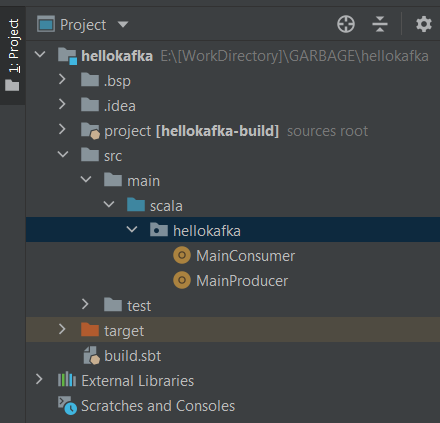
\includegraphics[scale=0.95]{figures/idea_kafka_scala_schema.png}
	\caption{ Структура проекта hellokafka }\label{fig:idea_kafka_scala_schema}
\end{figure}







\section{Spark Streaming и Kafka}


Затем (в самом простом варианте) следует создать продюсер (т.е. сервис порождающий данные) и консьюмер (т.е. сервис потребляющий данные).

Простой пример подписки на один топик
\begin{lstlisting}[
style = scala,
numbers = none	
]
val df = spark
  .readStream
  .format("kafka")
  .option("kafka.bootstrap.servers", "localhost:9092")
  .option("subscribe", "quickstart-events") // <-
  .load()
  
df.selectExpr("CAST(key AS STRING)", "CAST(value AS STRING)")
  .writeStream
  .outputMode("append")
  .format("console")
  .start().awaitTermination()
\end{lstlisting}



\section{Распределенное глубокое обучение с Elephas}

Elephas \url{https://github.com/maxpumperla/elephas} -- это распределенная платформа глубокого обучения, построенная на связке <<Keras + Spark>>.

Пример
\begin{lstlisting}[
style = ironpython,
numbers = none	
]
from pyspark import SparkContext, SparkConf
from keras.models import Sequential
from keras.layers.core import Dense, Dropout, Activation
from keras.optimizers import SGD
from elephas.utils.rdd_utils import to_simple_rdd
from elephas.spark_model import SparkModel

conf = SparkConf().setAppName("Elephas_App").setMaster("local[8]")
sc = SparkContext(conf = conf)

model = Sequential()
model.add(Dense(128, input_dim=784))
model.add(Activation("relu"))
model.add(Dropout(0.2))
model.add(Dense(128))
model.add(Activation("relu"))
model.add(Dropout(0.2))
model.add(Dense(10))
model.add(Activation("softmax"))
model.compile(loss="category_crossentropy", optimizer=SGD())

# RDD-подход
rdd = to_simple_rdd(sc, x_train, y_train)
spark_model = SparkModel(model, frequency="epoch")
spark_model.fit(rdd, epochs=20, batch_size=32, verbose=0, validation_split=0.1)

# DataFrame-подход. Лучше так!!!
df = to_data_frame(sc, x_train, y_train, categorical=True)
test_df = to_data_frame(sc, x_test, y_test, categorical=True)
estimator = ElephasEstimator(model, epochs=epochs, batch_size=batch_size, frequency="batch", categorical=True, nb_classes=nb_classes)
fitted_model = estimator.fit(df)
\end{lstlisting}

\section{Spark и Microsoft Machine Learning}

Очень полезная обертка для Spark \url{https://github.com/Azure/mmlspark}. 
Jupyter Notebook с примерами: \url{https://github.com/Azure/mmlspark/tree/master/notebooks/samples}

Запустить сессию на Python
\begin{lstlisting}[
style = ironpython,
numbers = none	
]
import pyspark
spark = pyspark.sql.SparkSession.builder.appName("MyApp") \
    .config("spark.jars.packages", "com.microsoft.ml.spark:mmlspark_2.11:1.0.0-rc3") \
    .config("spark.jars.repositories", "https://mmlspark.azureedge.net/maven") \
    .getOrCreate()
import mmlspark
\end{lstlisting}


\section{Ошибка java.lang.IllegalAccessException}

Ошибка \texttt{java.lang.IllegalAccessException} возникает (по моим наблюдениям), когда в преобразовании приходится обращаться к объекту, который (судя по всему) доступен только на драйвере
\begin{lstlisting}[
style = scala,
numbers = none	
]
val sortedCol: org.apache.spark.rdd.RDD[(Double, Long)] = ...

val ranksOnly = sortedCol.filter{
  val ranks = List[Long](...) // во избежание ошибки должен располагаться внутри преобразования
  elem => ranks.contains(elem._2) // здесь нельзя использовать case!!!
}
\end{lstlisting}




\section{Структурный и непрерывный стриминг}

Чем больше интервал пакетирования (размер батча), тем лучше (от нескольких миллисекунд до нескольких минут или даже часов).

Можно выделить три основных режима: 
\begin{itemize}
	\item микробатчевый режим (обычный DStream),
	
	\item структурированный микробатчевый,
	
	\item структурированный непрерывный.
\end{itemize}

Различают следующие модели:
\begin{itemize}
	\item Spark Streaming (DStream, микробатчевый режим) (не развивается!): это абстракция высокого уровня, называемая \emph{дискретным потоком} (DStream); представлен как последовательность RDD,
	
	\item Structured Streaming: передача не материализует всю таблицу сразу. Можно работать как с реляционной таблицей, которая обновляется в реальном времени. Structured Streaming считывает последние доступные данные из источника потоковых данных, обрабатывает их постепенно для обновления таблицы результатов, а затем отбрасывает первые данные. В этой модели Spark отвечает за обновление таблицы результатов при появлении новых данных. Не нужно думать об абстрактной ширине окна и т.д. как в случае DStream. 
\end{itemize}

Пример \emph{потокового запроса} (Streaming Query)
\begin{lstlisting}[
style = scala,
numbers = none	
]
events.where("state = CA").groupBy(window("time", "30 seconds")).avg("latency")
\end{lstlisting}

Области применения фреймверков:
\begin{itemize}
	\item Большой поток, простой агрегат: Spark,
	
	\item Быстрая реакция, сложный агрегат (поиск аномалий во входящих данных с датчиков): Flink,
	
	\item Минимум зависимостей, деплой в Kubernetes (микро-сервис, считающий статистику в реалтайме): Kafka
\end{itemize}


\section{Оптимизация гиперпараметров и AutoML}

Есть интересное расширение для \texttt{Spark ML} под именем \texttt{PravdaML}. Это расширение добавляет гибкости в вопросах организации потока данных, повышает коэффициент утилизации ресурсов и улучшения масштабирования ML.

\section{Apache Zookeeper}

\subsection{Общие сведения}

{Apache Zookeeper} -- это сервис распределенной координации -- централизованная служба для поддержки информации о конфигурации, обеспечения распределенной синхронизации и предоставления групповых служб. Все эти виды услуг используются в той или иной форме распределенными приложениями.

В конце сеанса следует:
\begin{itemize}
	\item Остановить продюсер, консамер с помощью \texttt{Ctrl-C},
	
	\item Остановить Kafka с помощью \texttt{Ctrl-C},
	
	\item Остановить ZooKeeper с помощью \texttt{Ctrl-C}.
\end{itemize}

Основные свойства Zookeeper:
\begin{itemize}
	\item пространство ключей образует дерево (иерархию, подобную файловой системе),
	
	\item значения могут содержаться в любом узле иерархии, а не только в листьях (как если бы файлы одновременно были бы и каталогами), узел иерархии называется znode,
	
	\item между клиентом и сервером двунаправленная связь, следовательно, клиент может подписываться как изменение конкретного значения или части иерархии,
	
	\item возможно создать временную пару ключ/значение, которая существует, пока клиент, ее создавший, подключен к серверу,
	
	\item все данные должны помещаться в память,
	
	\item устойчивость к смерти некритического количества узлов кластера.
\end{itemize}

\subsection{Установка и запуск Zookeeper}\label{subsec:zookeeper}

Чтобы установить Zookeeper на MacOS следует с официального сайта проекта скачать tar-архив \url{https://www.apache.org/dyn/closer.lua/zookeeper/zookeeper-3.6.2/apache-zookeeper-3.6.2-bin.tar.gz} и распаковать его, например, в поддиректорию \texttt{zookeeper} домашней директории
\begin{lstlisting}[
style = bash,
numbers = none	
]
tar -xvzf apache-zookeeper-3.6.2-bin &&\
mv apache-zookeeper-3.6.2 zookeeper-3.6.2
\end{lstlisting}

Затем нужно в конфигурационном файле командной оболочки \texttt{.bashrc}, \texttt{.zshrc} создать переменную окружения \texttt{ZOOKEEPER\_HOME}
\begin{lstlisting}[
title = {\sffamily \~{}/.zshrc},
style = bash,
numbers = none	
]
export ZOOKEEPER_HOME="/Users/leor.finkelberg/zookeeper/zookeeper-3.6.2/bin"
export PATH="$ZOOKEEPER_HOME:${PATH}"
\end{lstlisting}

Кроме того необходимо переименовать файл \texttt{zoo\_sample.cfg} в \texttt{zoo.cfg}, а затем заменить значение по умолчанию параметра \texttt{dataDir} на следующее \url{https://zookeeper.apache.org/doc/current/zookeeperStarted.html}
\begin{lstlisting}[
title = {\sffamily \~{}/zookeeper/zookeeper-3.6.2/conf/zoo.cfg},
style = bash,
numbers = none	
]
# каталог data должен существовать, иначе Zookeeper не сможет запустить сервер
dataDir=~/zookeeper/zookeeper-3.6.2/data
\end{lstlisting}
Остальные два параметра минимальной конфигурации -- \texttt{tickTime} и \texttt{clientPort} -- оставим без изменений.

Теперь можно запустить ZooKeeper
\begin{lstlisting}[
style = bash,
numbers = none	
]
zkServer.sh start 
\end{lstlisting}

Описанные выше шаги запускают ZooKeeper в автономном режиме. В этом случае не поддерживается репликация и если процесс упадет, то служба выйдет из строя. Такой схемы достаточно для большинства ситуаций, но все же, если требуется запустить ZooKeeper с поддержкой репликации, то следует ознакомиться с \url{https://zookeeper.apache.org/doc/current/zookeeperStarted.html#sc_RunningReplicatedZooKeeper}.

Далее устанавливаем соединение с ZooKeeper
\begin{lstlisting}[
style = bash,
numbers = none	
]
zkCli.sh -server 127.0.0.1:2181
\end{lstlisting}

Теперь нужно подготовить запуск Apache Kafka. Предварительно бинарные файлы можно скачать здесь \url{https://kafka.apache.org/downloads}.

Перед запуском Kafka следует указать куда будут писаться логи. Сделать это можно, изменив значение параметра \texttt{log.dirs} в файле \texttt{server.properties}
\begin{lstlisting}[
title = {\sffamily \~{}/kafka/kafka\_2.13-2.7.0/config/server.properties},
style = bash,
numbers = none
]
log.dirs=~/kafka/kafka_2.13-2.7.0/kafka-logs
\end{lstlisting}
и здесь же правим файл \texttt{zookeeper.properties}
\begin{lstlisting}[
title = {\sffamily \~{}/kafka/kafka\_2.13-2.7.0/config/zookeeper.properties},
style = bash,
numbers = none	
]
dataDir=~/kafka/kafka_2.13-2.7.0/zookeeper-data
\end{lstlisting}

А вот теперь можно запускать kafka-сессию
\begin{lstlisting}[
style = bash,
numbers = none	
]
./kafka-server-start.sh ~/kafka/kafka_2.13-2.7.0/config/server.properties
\end{lstlisting}

Для создания топика используем следующий сценарий командной оболочки
\begin{lstlisting}[
style = bash,
numbers = none	
]
./kafka-topics.sh --create --topic quickstart-events --bootstrap-server localhost:9092
# Created topic quickstart-events.
\end{lstlisting}

Посмотреть описание топика можно следующим образом
\begin{lstlisting}[
style = bash,
numbers = none	
]
./kafka-topics.sh --describe --topic quickstart-events --bootstrap-server localhost:9092
\end{lstlisting}

Клиент Kafka общается с брокерами сообщений через сеть для записи (или чтения) событий. Получив сообщение брокеры будут хранить его так долго, как это нужно. Запустим клиент продюсера, чтобы записать в топик несколько событий
\begin{lstlisting}[
style = bash,
numbers = none	
]
# запись некоторых событий в топик
./kafka-console-producer.sh --topic quickstart-events --bootstrap-server localhost:9092
>This is my first event
>This is my second events
>^C% # Ctrl-C
\end{lstlisting}

Теперь можно открыть еще один терминал и прочитать переданные в топик события
\begin{lstlisting}[
style = bash,
numbers = none
]
# чтение событий из топика
./kafka-console-consumer.sh --topic quickstart-events --from-beginning --bootstrap-server localhost:9092
# Ctrl-C
\end{lstlisting}

Остановить ZooKeeper можно так
\begin{lstlisting}[
style = bash,
numbers = none	
]
zkServer.sh stop
\end{lstlisting}




\section{Apache Kafka}\label{sec:kafka}

\subsection{Установка и запуск Kafka}

ВАЖНО: перед запуском Kafka следует запустить ZooKeeper (см.~\ref{subsec:zookeeper}).

Apache Kafka -- брокер сообщений, работающий поверх сервиса Apache Zookeeper.

Простая схема: создается топик (тема), в которую будут отправляться сообщения от продюсеров, и на которую смогут подписаться консьюмеры, чтобы их получать.

Для оперативного мониторинга Kafka лучше использовать Cluster Manager for Apache Kafka (CMAK) \url{https://github.com/yahoo/CMAK}.

\subsection{Общие сведения}

Очень полезное видео \url{https://www.youtube.com/watch?v=m5CDfrQLzrs}.

Очень полезный ресурс, на котором обсуждаются тонкие вопросы по работе с Kafka, которых нет даже в документации: \url{https://cwiki.apache.org/confluence/display/KAFKA/Kafka+Improvement+Proposals}.

Kafka -- брокер сообщений. Основная задача -- это доставка сообщений от продюсеров (сервисы, порождающие данные) до консьюмеров (сервисы, потребляющие данные).

Кластер Kafka почти всегда состоит из \emph{нод}, которые называют \emph{брокерами}, а координация между нодами осуществляется с помощью демона Zookeeper (см. \pic{fig:base_schema_kafka}).

\begin{figure}[h]
	\centering
	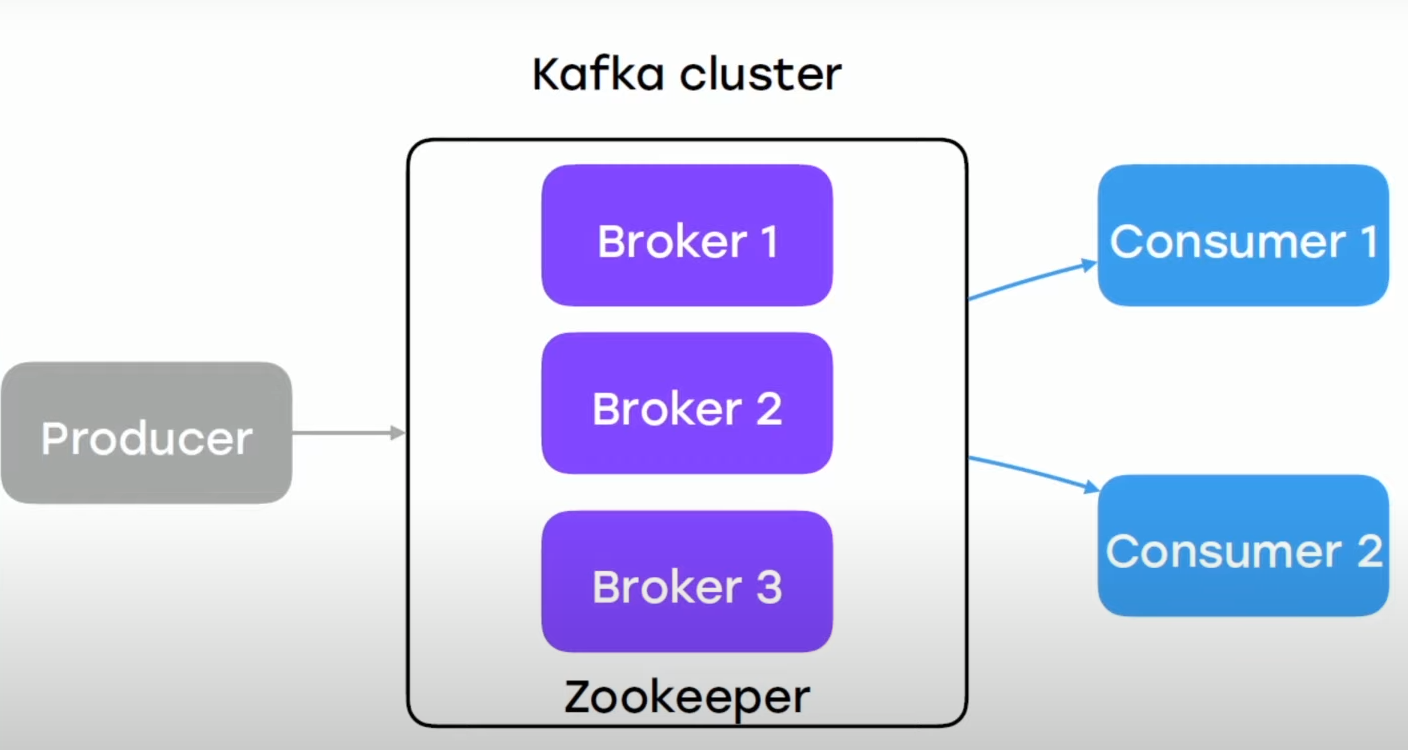
\includegraphics[scale=0.55]{figures/base_schema_kafka.png}
	\caption{ Базовая схема кластера Kafka }\label{fig:base_schema_kafka}
\end{figure}

Данные в Kafka разбиты по \emph{топикам} и каждый топик состоит из определенного числа \emph{партиций}. Топик находится на брокере. Партиция -- основная единица хранения данных в Kafka. Именно в партициях хранятся данные. Топик -- это логический контейнер вокруг партиции. Каждая партиция -- неизменяемая последовательность записей.

Продюсер может записывать данные только в конец очереди и никак не может повлиять на уже записанные данные (не может ни удалить, ни изменить). Каждому сообщению присваивается уникальный в пределах партиции порядковый номер (называет offset).

Как читать:
\begin{itemize}
	\item указываем потребителю топик, указываем номер партиции и указываем offset, с которого надо начать читать. Когда партиция исчерпается, потребитель будет ждать новых сообщений (в этом случае нужно вне Kafka запоминать offset),
	
	\item можно создать группу (groupId) и тогда Kafka будет сама следить за offset.
\end{itemize}

Продюсер \underline{всегда} пишет в \emph{лидер} (это брокер, т.е. узел кластера Kafka). Консьюмеры читают тоже с лидера (реплики нужны для подстраховки, т.е. если с лидером что-то происходит, то они займут его место).

Для одних партиций какой-то брокер является лидером, а для других он будет репликой!!!

ВАЖНО: даже после того как сообщение будет записано продюсером в лидер, оно не будет сразу же доступно для чтения консьюмерам. Сообщение будет доступно для чтения только после того как это сообщение <<подтянут>> \underline{все} реплики!!! Обойти это в Kafka нельзя. То есть нельзя сказать, например, что <<пусть сообщение считается доступным сразу после того как будет записано в лидер>>.

Данные пишутся со скоростью самого медленного брокера.

Для увеличения скорости записи, можно уменьшить значение параметра \texttt{replica.fetch.wait.max.ms} (это временной интервал, через который брокер-реплика будет опрашивать брокер-лидера). По умолчанию стоит 500 мс. Можно уменьшить до 200 мс.

Важный конфигурационный параметр -- \texttt{acks} (тип подтверждения, который будут получать от лидера при записи данных):
\begin{itemize}
	\item \texttt{acks=0}: не ждем никакого подтверждения; очень вероятна потеря сообщений (мы об этом никогда не узнаем); не подходит для важных данных,
	
	\item \texttt{acks=1}: ждем подтверждение только от лидера, что он записал у себя сообщение; не подходит для важных данных,
	
	\item \texttt{acks=-1}: ждем подтверждение от всех реплик (подходит). 
\end{itemize}

Параметр \texttt{replica.max.lag.ms=10000} (10 сек!): если реплика выпала, лидер будет ожидать ее 10 сек (это очень долго!!!). Можно уменьшить до 1 сек.

Параметр \texttt{min.insync.replicas} (очень важный параметр!!!) определяет минимальное число реплик в статусе \texttt{insync} (включая лидера), которое необходимо для успешной записи. По умолчанию стоит 1, но практичнее выставить 2. Этот параметр работает только для \texttt{acks=-1}.

Чтобы принудительно назначить брокер-реплику со статусом <<out of sync>> лидером, нужно в настройках топика задать \texttt{unclean.leader.election.enable=true}. Этот параметр бывает нужен, когда требуется что-то починить. В Kafka >=2.0.0 можно изменять динамически. Без понимания работы этого параметра лучше оставить значение по умолчанию, т.е. \texttt{false}.

Для того чтобы обеспечить и доступность и надежность в кластере из 3 брокеров следует использовать фактор репликации \texttt{Rf=3}, а \texttt{minISR=2}. В этом случае может возникнуть сложности с производительностью (в случае, если один из брокеров выпадет, нагрузка на оставшиеся может быть значительной со всеми вытекающими последствиями).

Иногда рекомендуют строить кластер из 5 брокеров (см. \pic{fig:cluster5brokers}): можно использовать \texttt{Rf=3}, \texttt{minISR=2}.

\begin{figure}[h]
	\centering
	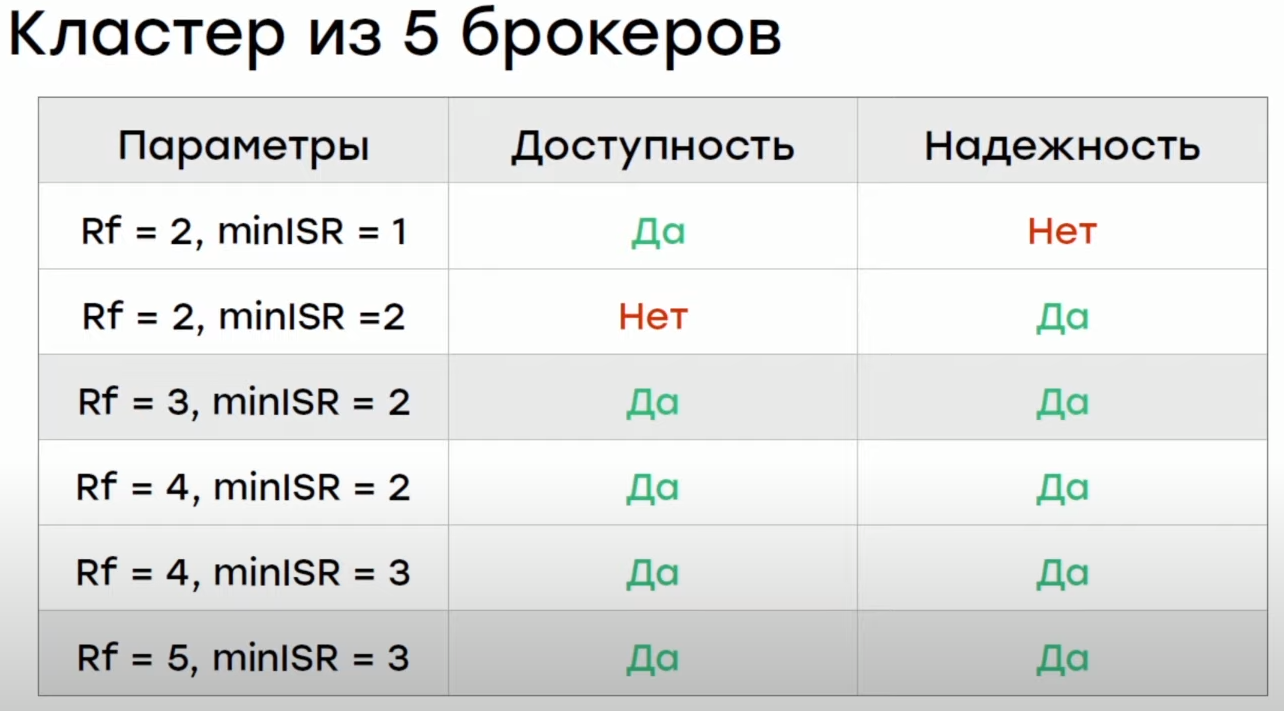
\includegraphics[scale=0.55]{figures/cluster5brokers.png}
	\caption{ Доступность и надежность кластера из 5 брокеров }\label{fig:cluster5brokers}
\end{figure}

В 3 ноды Zookeeper в отдельном кластере.

Выводы:
\begin{itemize}
	\item Kafka не автопилотируемый проект; за ней нужно постоянно следить,
	
	\item Надежная запись: \texttt{acks=-1} и \texttt{minISR > 2},
	
	\item Мониторинг + учения,
	
	\item Регулярные обновления,
	
	\item KIP и Jira очень полезны.
\end{itemize}


\section{Apache HBase}

HBase -- распределенная нереляционная (столбцово-ориентирования) база данных формата <<ключ-значение>>. 

\subsection{Установка и запуск}

Подробности, связанные с установкой различных режимах (автономном, распределенном и т.д.) можно узнать на странице \url{https://hbase.apache.org/book.html}.

Скачать tar-архив можно здесь \url{https://www.apache.org/dyn/closer.lua/hbase/2.4.0/hbase-2.4.0-bin.tar.gz}
\begin{lstlisting}[
style = bash,
numbers = none	
]
curl -O https://apache-mirror.rbc.ru/pub/apache/hbase/2.4.0/hbase-2.4.0-bin.tar.gz
\end{lstlisting}

Теперь следует распоковать архив
\begin{lstlisting}[
style = bash,
numbers = none	
]
tar -xvzf hbase-2.4.0...
\end{lstlisting}
перейти в директорию \directory{hbase-2.4.0} и задать путь до java в файле \texttt{hbase-env.sh}, раскоментировав нужную строку
\begin{lstlisting}[
title = {\sffamily conf/hbase-env.sh},
style = bash,
numbers = none	
]
export JAVA_HOME=/usr/local/Cellar/openjdk/15.0.1
\end{lstlisting}

В конфигурационном файле команданой оболочки удобно задать переменные окружения для Java и HBase
\begin{lstlisting}[
title = {\sffamily \~{}/.zshrc},
style = bash,
numbers = none	
]
# for HBase
export JAVA_HOME="/usr/local/Cellar/openjdk/15.0.1"
export PATH="${PATH}:/Users/leor.finkelberg/hbase/hbase-2.4.0/bin"
\end{lstlisting}

Диреткорию размещения java на MacOS X следует искать с помощью менеджера пакетов \texttt{brew}
\begin{lstlisting}[
style = bash,
numbers = none
]
brew list java # /usr/local/Cellar/openjdk/15.0.1/bin/java
\end{lstlisting}

ВАЖНО: обновить java, можно скачав соответствующую версию с ресурса \url{https://www.oracle.com/java/technologies/javase-jdk15-downloads.html}.

Запустить HBase можно с помощью сценария командной оболочки из \directory{bin/}
\begin{lstlisting}[
style = bash,
numbers = none	
]
start-hbase.sh
\end{lstlisting}

Подключиться к запущенному экземпляру можно так
\begin{lstlisting}[
style = bash,
numbers = none	
]
hbase shell
\end{lstlisting}

Для того чтобы убедиться, что процесс HMaster запущен можно воспользоваться утилитой~\texttt{jps}.

Бывает удобно следить за работой приложения с помощью Web-интерфейса, доступного на \url{http://localhost:16010}.

Закончить сессию можно с помощью команды \texttt{quit}. Затем нужно остановить HBase
\begin{lstlisting}[
style = bash,
numbers = none
]
stop-hbase.sh
\end{lstlisting}




\section{Пакетная и потоковая обработка данных}

Пакетная обработка -- обработка всего за раз без взаимодействия с конечным пользователем. Задача выполняется однократно или по расписанию, тригеру и пр.

Инструменты \emph{пакетной} обработки:
\begin{itemize}
	\item Spark -- стандарт в этой области,
	
	\item Flink -- псевдо-batch,
	
	\item Hive -- когда знаешь только SQL.
\end{itemize}

Инструменты \emph{потоковой} обработки:
\begin{itemize}
	\item Spark Streaming -- микробатчи,
	
	\item Flink -- реальный стириминг,
	
	\item Kafka Streams -- Kappa-архитектура.
\end{itemize}

Apache Kafka -- это быстрая, масштабируемая, надежная и отказоустойчивая система обмена сообщениями по механизму публикация-подписка. Еще можно сказать, что Kafka это распределенная потоковая платформа.

Если упрощенно, то Kafka предназначена для организации обмена сообщениями и результатами работы между микросервисами приложения.

Kafka работает с другими распределенными фреймверками как Spark, Samza, Flink для анализа и визуализации потоковых данных в реальном времени. Kafka хорошо интегрируется с ML фреймверками для решения ML/AI задач на потоках.

Основные определения:
\begin{itemize}
	\item Producer -- сервис, отправляющий сообщение,
	
	\item Consumer -- сервис, получающий данные,
	
	\item Broker -- один узел Kafka,
	
	\item Topic -- логическая очередь,
	
	\item Partition -- физическая часть очереди.
\end{itemize}

Обычно взаимодействие Kafka и Spark Streaming устроено следующим образом:
\begin{itemize}
	\item исходные данные записываются в топики Apache Kafka,
	
	\item приложение Spark Streaming считывает нужные данные и обрабатывает их согласно бизнес-логике,
	
	\item полученные результаты приложение Spark Streaming отправляет в место назначения -- новый топик Apache Kafka, озеро данных на базе Hadoop HDFS, аналитическую СУБД (HBase, Hive, Greenplum etc.) или BI-систему.
\end{itemize}

Топик состоит из партиций. Партиция упорядоченная и неизменяемая последовательность сообщений.

Семантика доставки:
\begin{itemize}
	\item At most once (максимум один раз) -- сообщения могут потеряны, но никогда не будут доставлены повторно (не будет дубликатов),
	
	\item At least once (минимум один раз) -- сообщения никогда не теряются, но могут быть доставлены повторно (возможны дубликаты),
	
	\item Exactly once (строго один раз) -- это то, чего на самом деле хотят люди; каждое сообщение доставляется только один раз.
\end{itemize}

Концепция и основные компоненты потоковой обработки
\begin{itemize}
	\item Structured Streaming -- передача не материализует всю таблицу сразу,
	
	\item Spark Streaming (Dstream) -- предоставляет абстракцию высокого уровня, называемую дискретным потоком или DStream, которая представляет непрерывный поток данных. DStream -- последовательность RDD.
\end{itemize}

Триггеры в Spark Streaming:
\begin{itemize}
	\item Unspecified (по умолчанию) -- если параметр триггера не указан явно, то по умолчанию запрос будет выполняться в режиме micro-batch, в котором микропакеты будут сгенерированы, как только предыдущий микропакет завершит обработку,
	
	\item Fixed interval micro-batches -- запрос будет выполнятся в режиме микропакетов, в котором микропакеты будут запускаться через указанные пользователем интервалы,
	
	\item One-time micro-batch -- запрос будет выполнять только один микропакет для обработки всех доступных данных, а затем остановится самостоятельно,
	
	\item Continuous with fixed checkpoint interval (экспериментально) -- запрос будет выполняться в новом режиме непрерывной обработки с малой задержкой.
\end{itemize}

Интеграция Kafka в Spark Streaming:
\begin{itemize}
	\item Write Ahead Logs (WAL) для Kafka -- это гарантирует, что никакие данные, полученные из любых надежных источников данных (т.е. транзакционных источников, таких как Flume, Kafka и Kinesis), не будут потеряны из-за сбоев. Даже для ненадежных (т.е. нетранзакционных) иточников, таких как простые старые сокеты, это сводит к минимуму потерю данных.
	
	\item Direct API для Kafka -- это позволяет обрабатывать каждую запись Kafka ровно один раз, несмотря на сбои, без использования журналов предварительной записи. Это делает конвейеры Spark Streaming + Kafka более эффективными, обеспечивая гарантию отказоусточивости.
\end{itemize}


\section{Приемы работы со Spark в Apache Zeppelin}

\texttt{Apache Zeppelin} \url{http://zeppelin.apache.org/download.html} -- это многофункциональная интерактивная оболочка, которая позволяет выполнять запросы к различным источникам данных, обрабатывать и визуализировать результаты, а самое главное <<из коробки>> поддерживает \texttt{Spark}. Близкий аналог \texttt{Jupyter Notebook}, но \texttt{Zeppelin} больше ориентирован на работу с базами данных. Он использует концепцию <<интерпретаторов>> -- плагинов, которые обеспечивают бекенд для какого-либо языка и/или БД.

Проще всего запустить \texttt{Zeppelin} с помощью \texttt{Docker}
\begin{lstlisting}[
style = bash,
numbers = none
]
docker run -p 8080:8080 --rm --name zeppelin apache/zeppelin:0.9.0
# или так
docker run -p 8080:8080 --rm \
  -v $(pwd)/logs:/logs \
  -v $(pwd)/notebook:/notebook \
  -e ZEPPELIN_LOG_DIR='/logs' \
  -e ZEPPELIN_NOTEBOOK_DIR='/notebook' \
  --name zeppelin apache/zeppelin:0.9.0
\end{lstlisting}

Страница \texttt{Zeppelin} будет доступна в браузере \texttt{localhost:8080}.

Подробное руководство по работе с \texttt{Apache Zeppelin} можно найти по адресу \url{https://docs.arenadata.io/aaw/Zeppelin/index.html}.




% Источники в "Газовой промышленности" нумеруются по мере упоминания 
\begin{thebibliography}{99}\addcontentsline{toc}{section}{Список литературы}
	\bibitem{carey:spark-2015}{ \emph{Карау Х.}, Конвински Э., Венделл П., Захария М. Изучаем Spark: молниеносный анализ данных. -- М.: ДМК Пресс, 2015. -- 304 с. }
\end{thebibliography}

%\listoffigures\addcontentsline{toc}{section}{Список иллюстраций}

\end{document}
